\documentclass[11pt,a4paper]{article}

\usepackage{acl2015}
\usepackage{times}
\usepackage{url}
\usepackage{latexsym}
\usepackage{amsmath}
\usepackage{ifthen}
\usepackage{xspace}
\usepackage{booktabs}
\usepackage{algorithm}
\usepackage{algorithmicx}
\usepackage{scalerel}
\usepackage{array}
\usepackage[noend]{algpseudocode}
\usepackage[usenames,dvipsnames]{color}
\usepackage{tikz}
\usepackage[all]{nowidow}
\usetikzlibrary{trees,matrix}
\usepackage{afterpage}
\usepackage{multirow,color}
\newcommand{\trevor}[1]{{\color{Maroon}{\bf{Trevor says:}} \emph{#1}}}
\newcommand{\matthias}[1]{{\color{RedOrange}{\bf{Matthias says:}} \emph{#1}}}
\newcommand{\ehsan}[1]{{\color{Cerulean}{\bf{Ehsan says:}} \emph{#1}}}
\newcommand{\reza}[1]{{\color{Blue}{\bf{Reza says:}} \emph{#1}}}


\newcommand*\Let[2]{\State #1 $\gets$ #2}
\newcommand*\CSA{\textsc{Csa}\xspace}
\newcommand*\CST{\textsc{Cst}\xspace}
\algrenewcommand\algorithmicrequire{\textbf{Precondition:}}
\algrenewcommand\algorithmicensure{\textbf{Postcondition:}}

\newcommand{\ngram}{$n$gram\xspace}
\newcommand{\ngrams}{$n$grams\xspace}

\newcommand{\rooot}[1]{\text{root}(#1)}
\newcommand{\leaf}[2]{\text{leaf}(#1, #2)}
\newcommand{\size}[2]{\text{size}(#1, #2)}
\newcommand{\depth}[2]{\text{depth}(#1, #2)}
\newcommand{\degree}[2]{\text{degree}(#1, #2)}
\newcommand{\edge}[3]{\text{edge}(#1, #2, #3)}
\newcommand{\children}[2]{\text{children}(#1, #2)}
\newcommand{\parent}[2]{\text{parent}(#1, #2)}
\newcommand{\backwardsearch}[4]{\text{backward-search}(#1, [#2,#3], #4)}
\newcommand{\forwardsearch}[4]{\text{forward-search}(#1, [#2,#3], #4)} % I've abbreviated away depth, char_pos
\newcommand{\intervalsymbols}[3]{\text{interval-symbols}(#1, [#2,#3])}

\DeclareMathOperator*{\Bigcdot}{\scalerel*{\cdot}{\bigodot}}

\newcommand{\lb}[1]{\text{lb}(#1)}
\newcommand{\rb}[1]{\text{rb}(#1)}
\newcommand{\dotpat}{\Bigcdot \alpha}
\newcommand{\patdot}{\alpha \Bigcdot}
\newcommand{\dotpatdot}{\Bigcdot \alpha \Bigcdot}
\newcommand{\nlplus}[1]{N^{1+}(#1)} % note it's an little L not a 1
\newcommand{\nlplusfunc}[3]{\textsc{N1Plus}(#1, #2, #3)} % "
\newcommand{\nlplusbacklfunc}[3]{\textsc{N1PlusBack1}(#1, #2, #3)} % " ^ 2
\newcommand{\nlplusfrontbackfunc}[4]{\textsc{N1PlusFrontBack}(#1, #2, #3, #4)} % " 
\newcommand{\nlplusfrontbacklfunc}[3]{\textsc{N1PlusFrontBack1}(#1, #2, #3)} % "

\newcommand{\tf}{t_{\text{F}}}
\newcommand{\tr}{t_{\text{R}}}
\newcommand{\af}{a_{\text{F}}}
\newcommand{\ar}{a_{\text{R}}}
\newcommand{\nf}{n_{\text{F}}}
\newcommand{\nr}{n_{\text{R}}}
\newcommand{\nrfull}{n_{\text{R}}^{\text{all}}}
\newcommand{\nffull}{n_{\text{F}}^{\text{all}}}
\newcommand{\chf}{c_{\text{F}}}
\newcommand{\chr}{c_{\text{R}}}

\newcommand{\ws}{\textbf{w}}

\newcommand{\Order}[1]{O(#1)}

%-- Sizes
\newcommand\kb[1]{\mbox{$#1$\,kiB}}
\newcommand\mb[1]{\mbox{$#1$\,MiB}}
\newcommand\gb[1]{\mbox{$#1$\,GiB}}
\newcommand\tb[1]{\mbox{$#1$\,TiB}}

%-- Syms
\newcommand{\col}{\ensuremath{\mathcal{T}}}  % collection
\newcommand{\pattern}{\ensuremath{\mathcal{P}}}  % collection
\newcommand{\plen}{\ensuremath{m}}
\newcommand{\collen}{\ensuremath{n}} 
\newcommand{\alphabet}{\ensuremath{\Sigma}} 
\newcommand{\alphabetsize}{\ensuremath{\sigma}} 


%-- ALG/DS
\newcommand{\SA}{\mbox{\emph{SA}}}

\title{Compact, Efficient and Unlimited Capacity:
    Language Modelling with Compressed Suffix Trees}

\author{First Author \\
  Affiliation / Address line 1 \\
  Affiliation / Address line 2 \\
  Affiliation / Address line 3 \\
  {\tt email@domain} \\\And
  Second Author \\
  Affiliation / Address line 1 \\
  Affiliation / Address line 2 \\
  Affiliation / Address line 3 \\
  {\tt email@domain} \\}

\date{}

\begin{document}
\maketitle
\begin{abstract}
  Here goes the abstract.
\end{abstract}

\section{Introduction}
\label{sec-intro}
%Language modelling is the task of estimating the probability of sequences of words in a language.
Language models (LMs) are one of the major and large components in many modern NLP systems, 
e.g. machine translation \cite{koehn2010book} 
and automatic speech recognition \cite{rab93book}.
%
One approach for accurate language modeling is neural 
\cite{Bengio:2003:NPL,DBLP:conf/interspeech/MikolovKBCK10}, but another is  count-based 
\cite{chen1996empirical} to harness the power of more data.
%
%The predominant approach to count-based language modelling is the $n$gram model,
%where a typical LM can contain as many as several hundred billions of $n$grams XX.
%
To be useful, LMs need to be not only accurate but also fast and compact.
%
In this paper, we build  fast and compact high-order \ngram LMs
%, the predominant approach in count-based language modeling, 
using modern succinct data structures.

%where the probability of a sequence of words is decomposed based on the chain rule ad approximatedusing the Markov assumption XX. 
%A typical count-based LM can contain as many as several hundred billions of $n$grams
%In this paper, we build  fast and compact $n$gram LMs, the predominant approach in count-based language modeling, on web-scale corpora using modern succinct data structures.
%
%We show how to compactly index the text statistics needed by $n$gram language models, so that they can be queried efficiently to make the probabilities on the fly.       
%
%Importantly, the stored index and text statistics are kept intact for $n$gram LMs with different orders (i.e. the context size), hence allow to relax the
%Markov assumption made in these LMs by considering very large contexts.



Depending on the order and the training corpus size, a typical \ngram LM may contain as many as several hundred billions of \ngrams \cite{brants2007large},
so storage and query time become challenge.
% Trevor: raising important algorithmic questions regarding efficient storage and retreival
%
As always, there is a trade-off between accuracy, space, and time, with recent papers considering small but approximate  \emph{lossy} LMs 
\cite{Chazelle:2004:BFE:982792.982797,guthrie2010storing},
or \emph{loss-less}  not-small LMs \cite{stolcke2011srilm} where compression and tries 
\cite{Germann:2009:TPT:1621947.1621952,heafield2011kenlm,pauls2011faster}, 
suffix trees \cite{kennington2012suffix}, and LODUS trees 
\cite{sall11,DBLP:conf/acl/WatanabeTI09}  
have been used to further reduce the storage.
% Trevor: sentence needed on LREC paper -- the approach most similar to ours
% Trevor: and also SRI/Ken
However, none of these papers scale up to high-order  
\ngram LMs on large corpora due to their  memory and time constrints when learning the models.
%
%However, none of the state-of-the-art LM toolkits provides the opportunity of
%investigating the behaviour of high-order LMs  
% 
Being able to work with high-order  LMs and investigate their behaviour 
with different smoothing techniques on large corpora is important, but 
infeasible with current state-of-the-art LM toolkits\footnote{ 
%none of the state-of-the-art toolkits provides this opportunity\footnote{
Indeed, there is clearly evidence that training high-order \ngram
LMs with the right amount of data and smoothing technique is beneficial \cite{wood2011sequence}.
}. 

%In $n$gram LMs, the probability of a sequence of words is decomposed based on the chain rule 
%and approximated using the Markov assumption 
%$P(w_1,\ldots,w_{\ell}) \approx \prod_{i=1}^{\ell} P(w_i|w_{i-n+1}^{i-1})$. 
%
%The Markov assumption reduces the number of model parameters 
%(which translates to more robust parameter estimation and smaller storage) 
%at the cost of probabililty approximation due to strong independence assumptions. 
%
%Making the space requirements  and query time of high-order LMs reasonable,
%our approach leads to weakening the strong independence assumptions inherent in $n$gram LMs.
%
%It is well known that, due to power-law nature of natural language [Zipf], maximum likelihood 
%estimator significantly overfits the training corpora. 
%
%Therefore, we build the indices to efficiently retrieve the counts 
%our indices store raw frequency counts 
%needed to compute \emph{smoothed} $n$gram probabilities using Kneser-Kney (KN) smoothing, 
%a powerful technique with elegant statistical properties\footnote{Although 
%we focus on KN-smoothing in this paper, our approach can be used to index and retrieve 
%counts needed in other smoothing techniques as well [chen and goodman].} [kneser kney].  
 
We make use of recent advances in 
\emph{compressed suffix trees} (\CSTs) \cite{nv-csurv07} 
to build compact indices  
with reasonable query-time (\S\ref{sec-suffix}) 
for high-order  LMs and investigate their behaviour 
with Kneser-Kney (KN) smoothing,  
a powerful technique with elegant statistical properties\footnote{Although
we focus on KN-smoothing, our approach can be used to index and compute
counts needed in other smoothing techniques as well \cite{chen1996empirical}.}  
\cite{kneser1995improved}.
% 
The key quantities for computing probability under KN-LMs
are raw frequencies of \ngrams 
and occurrence counts, i.e. the number of different contexts 
in which an \ngram has 
occurred which is challenging to compute.
%
%The raw frequency counts are simple to compute, but occurrence counts 
%are challenging. 
%
Our first proposal consists of two \CSTs to compute count queries 
in KN-LM (\S\ref{sec-lmsdsl}). 
% 
We further show how to leverage count queries for shorter contexts in queries for 
longer contexts to speed up the computation of KN-smoothed probabilities on the fly 
(\S\ref{sec-dual-cst}).
%
Our second proposal consists of only one \emph{augmented} \CST, which 
further improves both the space and query-time of our first proposal (\S\ref{sec-single-cst}). 
% 

Experiments ....
% Trevor: the experiments show that this approach matches the results of SRILM, while consuming a static memory footprint and construction cost irrespective of the \ngram order
% Trevor: futher, this allows us to run with unlimited markov order, which while slower than optimised low order models like \SRILM augurs well for future developments.
% Trevor: illustrate the scaling benefits of the model by building a character level LM over wikipedia, in only a few hours and modest memory footprint of a few GB
% Trevor: this work serves as a proof of concept, namely that high order language modelling is possible, and suitable for further optimisation to yield transformative tools for natural language processing.

%The predominant approach to count-based language modelling is the $n$gram model, where a typical LM can contain as many as several hundred billions of $n$grams XX.

%A typical LM can contain as many as severl hundred billions of $n$gramsFor modern NLP systems 
%The predominanr approach in language modelling is the $n$gram model, where the probability of a sequence of words is decomposed based on the chain rule and
%approximated using the Markov assumption XX. 
%

%The dominant approach to language modelling is $n$gram  model, where 

%LMs important, critical aspects are speed and scale. One avenue of better LMs using NN; another
%better count based LMs to harness more data (e.g., stupid backoff). 

%We're the latter, but marrying large scale with KN smoothing (better method). Crux is how to compute
%the quantities (counts, occ counts). 

%Suffix trees / arrays / tries etc used in the past. Either precomputed (KLM/SRI) or on the fly (slow
%LREC paper). But doesn't scale. We propose compressed SA/ST methods, which scale to massive datasets.

%Brief outline of how the method works; using one or two suffix trees. Forward/backward search.

%Pata on experiments: pplx good; can scale to large n and massive corpora; adequate runtime
%performance, around 100x slower than SRILM. Reranking gains? Can we run with INFINITE order?



\section{Suffix-based Indexing}
\label{sec-suffix}

\subsection{Suffix Arrays and Suffix Trees}

Overview with pretty picture. E.g., character level CSA / CST for 
'a quick brown fox jumped over the lazy dog' or similar.

Including something on BWT \& self indexes.

Forward and backward search.

\subsection{Compressed Suffix Structures}

WT, nested brackets CST, rank/select etc. Wiener links even?


\section{Language Modelling}
\label{sec-lm}

\subsection{Kneser Ney Language Modelling}
\label{sec-lm}

%Background, mathematical formulation.

This paper presents an efficient \ngram language model (LM) using succinct indexes to encode the model's sufficient statistics. % in such a way that they can be stored using only a small memory footprint and accessed efficiently. 
Although our method is generally applicable to many LM variants, we focus on the Kneser-Ney LM~\cite{kneser1995improved}, specifically the interpolated variant described in \newcite{chen1996empirical}, which has been shown to outperform other $n$gram LMs and has become the de-facto standard.

Interpolated Kneser-Ney describes the conditional probability of a word $w_i$ conditioned on the context of $m-1$ preceeding words, $w_{i-m+1}^{i-1}$, as 
\begin{align}
P(w_i |& w_{i-m+1}^{i-1})=\frac{\max\left[c(w^{i}_{i-m+1}) - D_m,0\right]}{c(w^{i-1}_{i-m+1})} \nonumber \\
& \hspace{-6mm} +\frac{D_m \nlplus{w^{i-1}_{i-m-1}\Bigcdot} }{c(w^{i-1}_{i-m+1})}  P(w_i | w_{i-m+2}^{i-1}) ,  
\label{eq:high}
\end{align}
where \mbox{$\nlplus{w^{i-1}_{i-m-1}\Bigcdot} = |\{s: c(w^{i-m}_{i-m-1}s)>0\}|$} is the \emph{occurrence count}, defined as the number of word types observed following the pattern, and $D$ is a vector of \ngram specific discount parameters.
The highest order probability estimate in (\ref{eq:high}) interpolates a discounted frequency estimate with a $m-1$ order probability, defined as 
\begin{align}
\! P(w_i |& w_{i-k+1}^{i-1})
 = \frac{\max\left[\nlplus{\Bigcdot w_{i-k+1}^{i}} - D_k,0\right]}{\nlplus{\Bigcdot w_{i-k+1}^{i-1} \Bigcdot}} \nonumber \\
&+ \frac{D_k \nlplus{w_{i-k+1}^{i-1}\Bigcdot}}{\nlplus{\Bigcdot w_{i-k+1}^{i-1} \Bigcdot}} P(w_i | w_{i-k+2}^{i-1}) \, , \! \label{eq:mid}
\end{align}
for $1<k<m$. 
Note the difference between (\ref{eq:mid})~and~(\ref{eq:high}), in that the frequency counts are redefined as occurrence counts. 
The above equation is self-recursive, where each step shrinks the conditioning context by the least recent symbol. 
The recursion stops with unigram probabilities,
%\begin{align*}
%\label{eq:low}
%
$ P(w_i) = \nlplus{\Bigcdot w_i} / \nlplus{\Bigcdot\Bigcdot}$.
%\end{align*}
%\newcite{chen1996empirical} report maximum likelihood estimates for the discount parameters, as simple functions of the corpus statistics for \ngrams occuring 1--4 times or occuring in 1--4 unique left contents. 
% Note that many other LM methods are defined in a similar manner to interpolated Kneser-Ney, using similar counts and occurrence counts for \ngram patterns.
Modified Kneser-Ney, proposed by~\newcite{chen1996empirical}, typically outperforms interpolated Kneser-Ney by using context specific discount parameters.
The implementation of this with our data structures is straightforward in principle, but brings a few added complexities in terms of dynamic computing other types of occurrence counts, which we leave for future work.


%%% Local Variables: 
%%% mode: latex
%%% TeX-master: "cstlm"
%%% End: 


\section{Using \CSTs for KN Computation}
\label{sec-lmsdsl}
%Computing counts, N1+ of several flavours of different sized n-grams.

The central requirement for computing probabilities under a Kneser-Ney
language model boils down to computing two types of counts: raw
frequencies of \ngrams and occurrence counts, quantifying in how many different contexts the \ngram has occurred.%
\footnote{The need such counts is not specific to Kneser Ney, indeed
  many other smoothing variants for \ngram LMs impose similar
  requirements and could be computed straightforwardly using the algorithms below.}
By electing to store the corpus directly in a suffix tree, we need to
provide mechanisms for computing these counts as they are needed based
on querying the data structure.

\begin{table}
\begin{align*}
c(\text{keep in the town})  & \quad 1 \\
c(\text{keep in the}) & \quad 2 \\
\nlplus{\text{keep in the} \Bigcdot} & \quad 2 \\ \hline
\nlplus{\Bigcdot \text{in the town}} & \quad 1\\
\nlplus{\Bigcdot \text{in the} \Bigcdot} & \quad 2 \\
\nlplus{\text{in the} \Bigcdot} & \quad 2 \\ \hline
\nlplus{\Bigcdot \text{the town}} & \quad 1\\
\nlplus{\Bigcdot \text{the} \Bigcdot} & \quad 4 \\
\nlplus{\text{the} \Bigcdot} & \quad 4  \\ \hline
\nlplus{\Bigcdot \text{town}} & \quad 1 \\
\nlplus{\Bigcdot \Bigcdot} & \quad 13 \\ % would be 14 but we exclude #$ right?
\nlplus{\Bigcdot} & \quad 9  % exclude $ right?
\end{align*}
\caption{Counts required for computing $P(\text{town} | \text{keep in
    the})$, and their values. Horizontal lines show the different
  stages in the backoff computation.}
\end{table}

Raw frequency counts are the simplest to compute, requiring first
identifying the node in the suffix tree labelled with the query
\ngram, from which we can read off the node's \emph{size}, defined as the
distance between its left and right bounds (corresponding to the
number of descendents under the node). To illustrate, consider
searching for \emph{the night} in  Figure~\ref{fig-suffix-tree}, which
matches a node with two descendents (labelled 19 and 12), and thus the
\ngram has count 2. This is a simple $\Order{1}$ operation once the
node has been identified.

More problematic are the occurrence counts, which come in several
flavours: with the dot to the right of the pattern, $\nlplus{\patdot}$,
to the left,  $\nlplus{\dotpat}$, and on both sides
$\nlplus{\dotpatdot}$. The first of these can be handled easily, by
querying the \emph{degree} of the matching node in the suffix tree. E.g., 
\emph{keep in} has two child nodes in  Figure~\ref{fig-suffix-tree},  
and thus there are two unique contexts in
which it can occur, $\nlplus{\emph{keep in~}\Bigcdot}=2$. This follows naturally from the suffix tree
construction, all descendent nodes correspond to larger \ngrams with
same prefix, and each child edge extends the \ngram with a different
subsequent symbol. 

\begin{algorithm}[th]
  \caption{Compute one-sided occurrence counts, $\nlplus{\dotpat}$ or $\nlplus{\patdot}$ for pattern $\alpha$ 
    \label{alg:n1plus}}
  \begin{algorithmic}[1]
    \Require{node $n$ in \CST $t$ matches $\alpha$}
    \Function{N1Plus}{$t, n, \alpha$} %\Comment{ $t$ is either forward or reverse \CST}
        \Let{$o$}{$0$} %\Comment{yielding $\nlplus{\patdot}$ or $\nlplus{\dotpat}$, respectively}
        %\If{$\leaf{t}{n} \, \wedge \, \depth{t}{n} = |\alpha|$}
        \If{$\depth{t}{n} = |\alpha|$}
          \Let{$o$}{$\degree{t}{n}$}
        \Else
          \Let{$o$}{$1$}
        \EndIf
      \State \Return{$o$}
    \EndFunction
  \end{algorithmic}
\label{alg-nlplus}
\end{algorithm}

A similar line of reasoning applies to computing
$\nlplus{\dotpat}$. Assuming we also have a suffix tree representing
the \emph{reversed corpus}, we can easily identify the reversed pattern
\emph{in keep} and query the degree for the matching node. This
approach is illustrated in Algorithm~\ref{alg-nlplus}, where we first
test if the node matches the pattern completely, i.e., its
\emph{depth} corresponds to the pattern length, in which case we use
the degree;\footnote{There are some corner cases involving sentinels \#
  and \$, which aren't counted in computing unique contexts.
  Such tests have been omitted from the algorithms for clarity, hereinafter. On publication the
  source code will be released with the complete implementation of the
  algorithms.}
otherwise the pattern is a prefix of the node, and
therefore can only be followed by a single unique symbol. 
For instance, \emph{the keep} partly matches an edge in
Figure~\ref{fig-suffix-tree} as it can only be followed by \emph{in}.
Finally, note that to compute $\nlplus{\dotpat}$ then $t$ must be the reversed \CST,
while supplying the forward \CST will yield $\nlplus{\patdot}$. Although
conceptually simple, using both reversed and forward suffix trees incurs double the storage overhead,
and, as we will show below, requires considerable additional search
overhead to find nodes matching each \ngram pattern in both suffix trees. We show later
how we can avoid the need for the reversed suffix tree, giving rise to
lower memory requirements and faster runtime.

The final component of the Kneser-Ney LM computation is
$\nlplus{\dotpatdot}$, the number of unique contexts consider symbols
on both sides of the pattern. 
Clearly this does not map naturally to a simple suffix tree operation,
requiring a more complex approach.



\begin{algorithm*}
  \caption{Compute two-sided occurrence counts, $\nlplus{\dotpatdot}$ 
    \label{alg:n1plusfb}}
  \begin{algorithmic}[1]
    \Require{$\nf$ is the node in the forward \CST $\tf$ matching pattern $\alpha$}
    \Require{$\nr$ is the node in the reverse \CST $\tr$ matching pattern $\alpha$}
    \Function{N1PlusFrontBack}{$\tf, \nf, \tr, \nr, \alpha$} 
        \Let{$o$}{$0$}
        %\If{$\leaf{\tf}{\nf} \, \vee \, \depth{\tf}{\nf} > |\alpha|$}   \Comment{leaves and patterns internal to an edge}
        \Let{$d$}{$\depth{\tf}{\nf} >$}   
        \If{$d > |\alpha|$}   \Comment{patterns internal to an edge}
          \Let{$o$}{$\nlplusfunc{\tr}{\nr}{\dotpat}$} \Comment{have only one right context}
        \Else
           \For{$\chf \gets \children{\tf}{\nf}$} 
              \Let{$s$}{$\edge{\tf}{\chf}{d+1}$} \Comment{find the first symbol on the edge label}
              \Let{$\chr$}{$\backwardsearch{\ar}{\lb{\nr}}{\rb{\nr}}{s}$} \Comment{find child node in reverse \CST}
              \Statex    \Comment{$\ar$ is the \CSA component of $\tr$}
              \Let{$o$}{$o + \nlplusfunc{\tr}{\chr}{\dotpat s}$}
            \EndFor
        \EndIf
      \State \Return{$o$}
    \EndFunction
  \end{algorithmic}
\end{algorithm*}




\subsection{Dual \CST Algorithm} 

Algorithm overview.

Include paragraph on computing the discounts.

\subsection{Complexity Analysis}

\section{Improved single \CST approach}

Just show N1+fb algo; leave rest to supporting material.
%%% Local Variables: 
%%% mode: latex
%%% TeX-master: "cstlm"
%%% End: 


\section{Experiments}
\label{sec-experiments}
%
\paragraph{Datasets}
We used Europarl dataset and the data was numberized after tokenizing, splitting, and excluding xml markups. The first $10K$ sentences were used as the test data, and the last 80\% as the training data, giving rise to training corpora of between 8M and 50M tokens and binary encoding of word integers of up to 200MB (see \supp Table~4).
\trevor{Sentence on wikipedia}

%\begin{table}
%\resizebox{1\columnwidth}{!}{
%\begin{tabular}{ll|cc|c}
%Language&&Size (MB)&Tokens (M)& Sentences (K)\\
%\toprule 
%Bulgarian&BG&36.11&8.53&329\\
%Czech&CS&53.48&12.25&535\\
%German&DE&171.80&44.07&1785 \\
%English&EN&179.15&49.32&1815\\
%Finnish&FI&145.32&32.85&1737\\
%French&FR&197.68&53.82&1792\\
%Hungarian&HU&52.53&12.02&527\\
%Italian&IT&186.67&48.08&1703\\
%Portuguese&PT&187.20&49.03&1737\\
%\end{tabular}}
%\caption{Tokens and sentence counts refer to the training partition. \trevor{Move to \supp}}\label{fig:data}
%\end{table}

\begin{figure}[tb]
% Created by tikzDevice version 0.8.1 on 2015-05-29 13:08:13
% !TEX encoding = UTF-8 Unicode
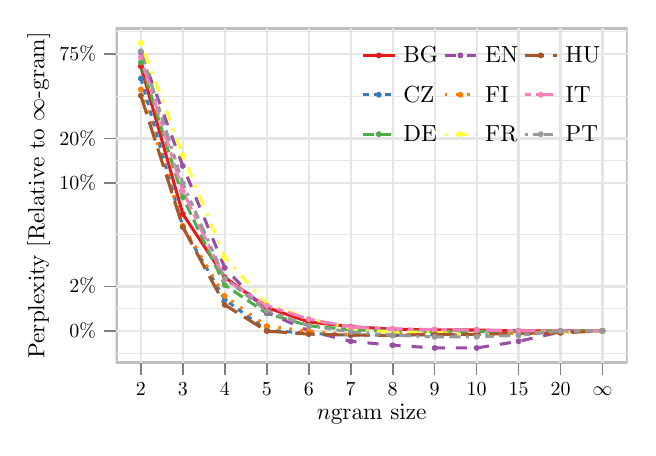
\begin{tikzpicture}[x=1pt,y=1pt]
\definecolor{fillColor}{RGB}{255,255,255}
\path[use as bounding box,fill=fillColor,fill opacity=0.00] (0,0) rectangle (216.81,144.54);
\begin{scope}
\path[clip] (  0.00,  0.00) rectangle (216.81,144.54);
\definecolor{fillColor}{RGB}{255,255,255}

\path[fill=fillColor] (  0.00,  0.00) rectangle (216.81,144.54);
\end{scope}
\begin{scope}
\path[clip] ( 31.80, 23.29) rectangle (216.81,144.54);
\definecolor{drawColor}{RGB}{190,190,190}

\path[draw=drawColor,line width= 1.5pt,line join=round,line cap=round] ( 31.80, 23.29) rectangle (216.81,144.54);
\definecolor{drawColor}{gray}{0.90}

\path[draw=drawColor,line width= 0.3pt,line join=round] ( 31.80, 26.94) --
	(216.81, 26.94);

\path[draw=drawColor,line width= 0.3pt,line join=round] ( 31.80, 43.01) --
	(216.81, 43.01);

\path[draw=drawColor,line width= 0.3pt,line join=round] ( 31.80, 69.72) --
	(216.81, 69.72);

\path[draw=drawColor,line width= 0.3pt,line join=round] ( 31.80, 96.43) --
	(216.81, 96.43);

\path[draw=drawColor,line width= 0.3pt,line join=round] ( 31.80,119.79) --
	(216.81,119.79);

\path[draw=drawColor,line width= 0.3pt,line join=round] ( 31.80,143.16) --
	(216.81,143.16);

\path[draw=drawColor,line width= 0.8pt,line join=round] ( 31.80, 34.98) --
	(216.81, 34.98);

\path[draw=drawColor,line width= 0.8pt,line join=round] ( 31.80, 51.05) --
	(216.81, 51.05);

\path[draw=drawColor,line width= 0.8pt,line join=round] ( 31.80, 88.39) --
	(216.81, 88.39);

\path[draw=drawColor,line width= 0.8pt,line join=round] ( 31.80,104.46) --
	(216.81,104.46);

\path[draw=drawColor,line width= 0.8pt,line join=round] ( 31.80,135.12) --
	(216.81,135.12);

\path[draw=drawColor,line width= 0.8pt,line join=round] ( 40.90, 23.29) --
	( 40.90,144.54);

\path[draw=drawColor,line width= 0.8pt,line join=round] ( 56.06, 23.29) --
	( 56.06,144.54);

\path[draw=drawColor,line width= 0.8pt,line join=round] ( 71.23, 23.29) --
	( 71.23,144.54);

\path[draw=drawColor,line width= 0.8pt,line join=round] ( 86.39, 23.29) --
	( 86.39,144.54);

\path[draw=drawColor,line width= 0.8pt,line join=round] (101.56, 23.29) --
	(101.56,144.54);

\path[draw=drawColor,line width= 0.8pt,line join=round] (116.72, 23.29) --
	(116.72,144.54);

\path[draw=drawColor,line width= 0.8pt,line join=round] (131.89, 23.29) --
	(131.89,144.54);

\path[draw=drawColor,line width= 0.8pt,line join=round] (147.05, 23.29) --
	(147.05,144.54);

\path[draw=drawColor,line width= 0.8pt,line join=round] (162.22, 23.29) --
	(162.22,144.54);

\path[draw=drawColor,line width= 0.8pt,line join=round] (177.38, 23.29) --
	(177.38,144.54);

\path[draw=drawColor,line width= 0.8pt,line join=round] (192.55, 23.29) --
	(192.55,144.54);

\path[draw=drawColor,line width= 0.8pt,line join=round] (207.71, 23.29) --
	(207.71,144.54);
\definecolor{drawColor}{RGB}{228,26,28}

\path[draw=drawColor,line width= 1.1pt,line join=round] ( 40.90,130.63) --
	( 56.06, 77.21) --
	( 71.23, 54.31) --
	( 86.39, 43.41) --
	(101.56, 38.23) --
	(116.72, 36.51) --
	(131.89, 35.60) --
	(147.05, 35.29) --
	(162.22, 35.29) --
	(177.38, 34.98) --
	(192.55, 34.98) --
	(207.71, 34.98);
\definecolor{drawColor}{RGB}{55,126,184}

\path[draw=drawColor,line width= 1.1pt,dash pattern=on 2pt off 2pt ,line join=round] ( 40.90,126.19) --
	( 56.06, 72.56) --
	( 71.23, 46.26) --
	( 86.39, 35.27) --
	(101.56, 34.06) --
	(116.72, 33.43) --
	(131.89, 33.43) --
	(147.05, 33.59) --
	(162.22, 33.59) --
	(177.38, 34.67) --
	(192.55, 34.82) --
	(207.71, 34.98);
\definecolor{drawColor}{RGB}{77,175,74}

\path[draw=drawColor,line width= 1.1pt,dash pattern=on 4pt off 2pt ,line join=round] ( 40.90,131.98) --
	( 56.06, 83.27) --
	( 71.23, 51.55) --
	( 86.39, 41.31) --
	(101.56, 36.83) --
	(116.72, 35.40) --
	(131.89, 34.98) --
	(147.05, 34.76) --
	(162.22, 34.76) --
	(177.38, 34.76) --
	(192.55, 34.98) --
	(207.71, 34.98);
\definecolor{drawColor}{RGB}{152,78,163}

\path[draw=drawColor,line width= 1.1pt,dash pattern=on 4pt off 4pt ,line join=round] ( 40.90,135.63) --
	( 56.06, 94.56) --
	( 71.23, 57.75) --
	( 86.39, 41.66) --
	(101.56, 34.98) --
	(116.72, 31.20) --
	(131.89, 29.79) --
	(147.05, 28.80) --
	(162.22, 28.80) --
	(177.38, 31.20) --
	(192.55, 34.58) --
	(207.71, 34.98);
\definecolor{drawColor}{RGB}{255,127,0}

\path[draw=drawColor,line width= 1.1pt,dash pattern=on 1pt off 3pt ,line join=round] ( 40.90,122.24) --
	( 56.06, 72.99) --
	( 71.23, 47.59) --
	( 86.39, 36.68) --
	(101.56, 34.90) --
	(116.72, 33.68) --
	(131.89, 33.76) --
	(147.05, 33.92) --
	(162.22, 33.53) --
	(177.38, 34.22) --
	(192.55, 34.75) --
	(207.71, 34.98);
\definecolor{drawColor}{RGB}{255,255,51}

\path[draw=drawColor,line width= 1.1pt,dash pattern=on 1pt off 3pt on 4pt off 3pt ,line join=round] ( 40.90,139.03) --
	( 56.06, 98.50) --
	( 71.23, 61.44) --
	( 86.39, 44.72) --
	(101.56, 39.37) --
	(116.72, 35.92) --
	(131.89, 34.49) --
	(147.05, 34.49) --
	(162.22, 33.48) --
	(177.38, 33.99) --
	(192.55, 34.49) --
	(207.71, 34.98);
\definecolor{drawColor}{RGB}{166,86,40}

\path[draw=drawColor,line width= 1.1pt,dash pattern=on 7pt off 3pt ,line join=round] ( 40.90,119.98) --
	( 56.06, 72.52) --
	( 71.23, 44.35) --
	( 86.39, 34.91) --
	(101.56, 33.80) --
	(116.72, 33.47) --
	(131.89, 33.36) --
	(147.05, 33.74) --
	(162.22, 33.69) --
	(177.38, 34.07) --
	(192.55, 34.25) --
	(207.71, 34.98);
\definecolor{drawColor}{RGB}{247,129,191}

\path[draw=drawColor,line width= 1.1pt,dash pattern=on 2pt off 2pt on 6pt off 2pt ,line join=round] ( 40.90,133.85) --
	( 56.06, 85.45) --
	( 71.23, 53.61) --
	( 86.39, 44.06) --
	(101.56, 39.24) --
	(116.72, 36.33) --
	(131.89, 35.69) --
	(147.05, 35.50) --
	(162.22, 35.23) --
	(177.38, 35.00) --
	(192.55, 34.96) --
	(207.71, 34.98);
\definecolor{drawColor}{gray}{0.60}

\path[draw=drawColor,line width= 1.1pt,dash pattern=on 1pt off 2pt on 2pt off 2pt on 3pt off 2pt on 4pt off 2pt ,line join=round] ( 40.90,136.04) --
	( 56.06, 88.32) --
	( 71.23, 53.95) --
	( 86.39, 42.18) --
	(101.56, 36.86) --
	(116.72, 34.57) --
	(131.89, 33.40) --
	(147.05, 32.81) --
	(162.22, 32.85) --
	(177.38, 33.35) --
	(192.55, 34.90) --
	(207.71, 34.98);
\definecolor{fillColor}{RGB}{228,26,28}

\path[fill=fillColor] ( 40.90,130.63) circle (  1.07);

\path[fill=fillColor] ( 56.06, 77.21) circle (  1.07);

\path[fill=fillColor] ( 71.23, 54.31) circle (  1.07);

\path[fill=fillColor] ( 86.39, 43.41) circle (  1.07);

\path[fill=fillColor] (101.56, 38.23) circle (  1.07);

\path[fill=fillColor] (116.72, 36.51) circle (  1.07);

\path[fill=fillColor] (131.89, 35.60) circle (  1.07);

\path[fill=fillColor] (147.05, 35.29) circle (  1.07);

\path[fill=fillColor] (162.22, 35.29) circle (  1.07);

\path[fill=fillColor] (177.38, 34.98) circle (  1.07);

\path[fill=fillColor] (192.55, 34.98) circle (  1.07);

\path[fill=fillColor] (207.71, 34.98) circle (  1.07);
\definecolor{fillColor}{RGB}{55,126,184}

\path[fill=fillColor] ( 40.90,126.19) circle (  1.07);

\path[fill=fillColor] ( 56.06, 72.56) circle (  1.07);

\path[fill=fillColor] ( 71.23, 46.26) circle (  1.07);

\path[fill=fillColor] ( 86.39, 35.27) circle (  1.07);

\path[fill=fillColor] (101.56, 34.06) circle (  1.07);

\path[fill=fillColor] (116.72, 33.43) circle (  1.07);

\path[fill=fillColor] (131.89, 33.43) circle (  1.07);

\path[fill=fillColor] (147.05, 33.59) circle (  1.07);

\path[fill=fillColor] (162.22, 33.59) circle (  1.07);

\path[fill=fillColor] (177.38, 34.67) circle (  1.07);

\path[fill=fillColor] (192.55, 34.82) circle (  1.07);

\path[fill=fillColor] (207.71, 34.98) circle (  1.07);
\definecolor{fillColor}{RGB}{77,175,74}

\path[fill=fillColor] ( 40.90,131.98) circle (  1.07);

\path[fill=fillColor] ( 56.06, 83.27) circle (  1.07);

\path[fill=fillColor] ( 71.23, 51.55) circle (  1.07);

\path[fill=fillColor] ( 86.39, 41.31) circle (  1.07);

\path[fill=fillColor] (101.56, 36.83) circle (  1.07);

\path[fill=fillColor] (116.72, 35.40) circle (  1.07);

\path[fill=fillColor] (131.89, 34.98) circle (  1.07);

\path[fill=fillColor] (147.05, 34.76) circle (  1.07);

\path[fill=fillColor] (162.22, 34.76) circle (  1.07);

\path[fill=fillColor] (177.38, 34.76) circle (  1.07);

\path[fill=fillColor] (192.55, 34.98) circle (  1.07);

\path[fill=fillColor] (207.71, 34.98) circle (  1.07);
\definecolor{fillColor}{RGB}{152,78,163}

\path[fill=fillColor] ( 40.90,135.63) circle (  1.07);

\path[fill=fillColor] ( 56.06, 94.56) circle (  1.07);

\path[fill=fillColor] ( 71.23, 57.75) circle (  1.07);

\path[fill=fillColor] ( 86.39, 41.66) circle (  1.07);

\path[fill=fillColor] (101.56, 34.98) circle (  1.07);

\path[fill=fillColor] (116.72, 31.20) circle (  1.07);

\path[fill=fillColor] (131.89, 29.79) circle (  1.07);

\path[fill=fillColor] (147.05, 28.80) circle (  1.07);

\path[fill=fillColor] (162.22, 28.80) circle (  1.07);

\path[fill=fillColor] (177.38, 31.20) circle (  1.07);

\path[fill=fillColor] (192.55, 34.58) circle (  1.07);

\path[fill=fillColor] (207.71, 34.98) circle (  1.07);
\definecolor{fillColor}{RGB}{255,127,0}

\path[fill=fillColor] ( 40.90,122.24) circle (  1.07);

\path[fill=fillColor] ( 56.06, 72.99) circle (  1.07);

\path[fill=fillColor] ( 71.23, 47.59) circle (  1.07);

\path[fill=fillColor] ( 86.39, 36.68) circle (  1.07);

\path[fill=fillColor] (101.56, 34.90) circle (  1.07);

\path[fill=fillColor] (116.72, 33.68) circle (  1.07);

\path[fill=fillColor] (131.89, 33.76) circle (  1.07);

\path[fill=fillColor] (147.05, 33.92) circle (  1.07);

\path[fill=fillColor] (162.22, 33.53) circle (  1.07);

\path[fill=fillColor] (177.38, 34.22) circle (  1.07);

\path[fill=fillColor] (192.55, 34.75) circle (  1.07);

\path[fill=fillColor] (207.71, 34.98) circle (  1.07);
\definecolor{fillColor}{RGB}{255,255,51}

\path[fill=fillColor] ( 40.90,139.03) circle (  1.07);

\path[fill=fillColor] ( 56.06, 98.50) circle (  1.07);

\path[fill=fillColor] ( 71.23, 61.44) circle (  1.07);

\path[fill=fillColor] ( 86.39, 44.72) circle (  1.07);

\path[fill=fillColor] (101.56, 39.37) circle (  1.07);

\path[fill=fillColor] (116.72, 35.92) circle (  1.07);

\path[fill=fillColor] (131.89, 34.49) circle (  1.07);

\path[fill=fillColor] (147.05, 34.49) circle (  1.07);

\path[fill=fillColor] (162.22, 33.48) circle (  1.07);

\path[fill=fillColor] (177.38, 33.99) circle (  1.07);

\path[fill=fillColor] (192.55, 34.49) circle (  1.07);

\path[fill=fillColor] (207.71, 34.98) circle (  1.07);
\definecolor{fillColor}{RGB}{166,86,40}

\path[fill=fillColor] ( 40.90,119.98) circle (  1.07);

\path[fill=fillColor] ( 56.06, 72.52) circle (  1.07);

\path[fill=fillColor] ( 71.23, 44.35) circle (  1.07);

\path[fill=fillColor] ( 86.39, 34.91) circle (  1.07);

\path[fill=fillColor] (101.56, 33.80) circle (  1.07);

\path[fill=fillColor] (116.72, 33.47) circle (  1.07);

\path[fill=fillColor] (131.89, 33.36) circle (  1.07);

\path[fill=fillColor] (147.05, 33.74) circle (  1.07);

\path[fill=fillColor] (162.22, 33.69) circle (  1.07);

\path[fill=fillColor] (177.38, 34.07) circle (  1.07);

\path[fill=fillColor] (192.55, 34.25) circle (  1.07);

\path[fill=fillColor] (207.71, 34.98) circle (  1.07);
\definecolor{fillColor}{RGB}{247,129,191}

\path[fill=fillColor] ( 40.90,133.85) circle (  1.07);

\path[fill=fillColor] ( 56.06, 85.45) circle (  1.07);

\path[fill=fillColor] ( 71.23, 53.61) circle (  1.07);

\path[fill=fillColor] ( 86.39, 44.06) circle (  1.07);

\path[fill=fillColor] (101.56, 39.24) circle (  1.07);

\path[fill=fillColor] (116.72, 36.33) circle (  1.07);

\path[fill=fillColor] (131.89, 35.69) circle (  1.07);

\path[fill=fillColor] (147.05, 35.50) circle (  1.07);

\path[fill=fillColor] (162.22, 35.23) circle (  1.07);

\path[fill=fillColor] (177.38, 35.00) circle (  1.07);

\path[fill=fillColor] (192.55, 34.96) circle (  1.07);

\path[fill=fillColor] (207.71, 34.98) circle (  1.07);
\definecolor{fillColor}{gray}{0.60}

\path[fill=fillColor] ( 40.90,136.04) circle (  1.07);

\path[fill=fillColor] ( 56.06, 88.32) circle (  1.07);

\path[fill=fillColor] ( 71.23, 53.95) circle (  1.07);

\path[fill=fillColor] ( 86.39, 42.18) circle (  1.07);

\path[fill=fillColor] (101.56, 36.86) circle (  1.07);

\path[fill=fillColor] (116.72, 34.57) circle (  1.07);

\path[fill=fillColor] (131.89, 33.40) circle (  1.07);

\path[fill=fillColor] (147.05, 32.81) circle (  1.07);

\path[fill=fillColor] (162.22, 32.85) circle (  1.07);

\path[fill=fillColor] (177.38, 33.35) circle (  1.07);

\path[fill=fillColor] (192.55, 34.90) circle (  1.07);

\path[fill=fillColor] (207.71, 34.98) circle (  1.07);
\end{scope}
\begin{scope}
\path[clip] (  0.00,  0.00) rectangle (216.81,144.54);
\definecolor{drawColor}{RGB}{0,0,0}

\node[text=drawColor,anchor=base east,inner sep=0pt, outer sep=0pt, scale=  0.72] at ( 24.69, 32.63) {0\%};

\node[text=drawColor,anchor=base east,inner sep=0pt, outer sep=0pt, scale=  0.72] at ( 24.69, 48.71) {2\%};

\node[text=drawColor,anchor=base east,inner sep=0pt, outer sep=0pt, scale=  0.72] at ( 24.69, 86.04) {10\%};

\node[text=drawColor,anchor=base east,inner sep=0pt, outer sep=0pt, scale=  0.72] at ( 24.69,102.12) {20\%};

\node[text=drawColor,anchor=base east,inner sep=0pt, outer sep=0pt, scale=  0.72] at ( 24.69,132.78) {75\%};
\end{scope}
\begin{scope}
\path[clip] (  0.00,  0.00) rectangle (216.81,144.54);
\definecolor{drawColor}{gray}{0.50}

\path[draw=drawColor,line width= 0.6pt,line join=round] ( 27.53, 34.98) --
	( 31.80, 34.98);

\path[draw=drawColor,line width= 0.6pt,line join=round] ( 27.53, 51.05) --
	( 31.80, 51.05);

\path[draw=drawColor,line width= 0.6pt,line join=round] ( 27.53, 88.39) --
	( 31.80, 88.39);

\path[draw=drawColor,line width= 0.6pt,line join=round] ( 27.53,104.46) --
	( 31.80,104.46);

\path[draw=drawColor,line width= 0.6pt,line join=round] ( 27.53,135.12) --
	( 31.80,135.12);
\end{scope}
\begin{scope}
\path[clip] (  0.00,  0.00) rectangle (216.81,144.54);
\definecolor{drawColor}{gray}{0.50}

\path[draw=drawColor,line width= 0.6pt,line join=round] ( 40.90, 19.02) --
	( 40.90, 23.29);

\path[draw=drawColor,line width= 0.6pt,line join=round] ( 56.06, 19.02) --
	( 56.06, 23.29);

\path[draw=drawColor,line width= 0.6pt,line join=round] ( 71.23, 19.02) --
	( 71.23, 23.29);

\path[draw=drawColor,line width= 0.6pt,line join=round] ( 86.39, 19.02) --
	( 86.39, 23.29);

\path[draw=drawColor,line width= 0.6pt,line join=round] (101.56, 19.02) --
	(101.56, 23.29);

\path[draw=drawColor,line width= 0.6pt,line join=round] (116.72, 19.02) --
	(116.72, 23.29);

\path[draw=drawColor,line width= 0.6pt,line join=round] (131.89, 19.02) --
	(131.89, 23.29);

\path[draw=drawColor,line width= 0.6pt,line join=round] (147.05, 19.02) --
	(147.05, 23.29);

\path[draw=drawColor,line width= 0.6pt,line join=round] (162.22, 19.02) --
	(162.22, 23.29);

\path[draw=drawColor,line width= 0.6pt,line join=round] (177.38, 19.02) --
	(177.38, 23.29);

\path[draw=drawColor,line width= 0.6pt,line join=round] (192.55, 19.02) --
	(192.55, 23.29);

\path[draw=drawColor,line width= 0.6pt,line join=round] (207.71, 19.02) --
	(207.71, 23.29);
\end{scope}
\begin{scope}
\path[clip] (  0.00,  0.00) rectangle (216.81,144.54);
\definecolor{drawColor}{RGB}{0,0,0}

\node[text=drawColor,anchor=base,inner sep=0pt, outer sep=0pt, scale=  0.72] at ( 40.90, 11.49) {2};

\node[text=drawColor,anchor=base,inner sep=0pt, outer sep=0pt, scale=  0.72] at ( 56.06, 11.49) {3};

\node[text=drawColor,anchor=base,inner sep=0pt, outer sep=0pt, scale=  0.72] at ( 71.23, 11.49) {4};

\node[text=drawColor,anchor=base,inner sep=0pt, outer sep=0pt, scale=  0.72] at ( 86.39, 11.49) {5};

\node[text=drawColor,anchor=base,inner sep=0pt, outer sep=0pt, scale=  0.72] at (101.56, 11.49) {6};

\node[text=drawColor,anchor=base,inner sep=0pt, outer sep=0pt, scale=  0.72] at (116.72, 11.49) {7};

\node[text=drawColor,anchor=base,inner sep=0pt, outer sep=0pt, scale=  0.72] at (131.89, 11.49) {8};

\node[text=drawColor,anchor=base,inner sep=0pt, outer sep=0pt, scale=  0.72] at (147.05, 11.49) {9};

\node[text=drawColor,anchor=base,inner sep=0pt, outer sep=0pt, scale=  0.72] at (162.22, 11.49) {10};

\node[text=drawColor,anchor=base,inner sep=0pt, outer sep=0pt, scale=  0.72] at (177.38, 11.49) {15};

\node[text=drawColor,anchor=base,inner sep=0pt, outer sep=0pt, scale=  0.72] at (192.55, 11.49) {20};

\node[text=drawColor,anchor=base,inner sep=0pt, outer sep=0pt, scale=  0.72] at (207.71, 11.49) {$\infty$};
\end{scope}
\begin{scope}
\path[clip] (  0.00,  0.00) rectangle (216.81,144.54);
\definecolor{drawColor}{RGB}{0,0,0}

\node[text=drawColor,anchor=base,inner sep=0pt, outer sep=0pt, scale=  0.84] at (124.31,  3.01) {\ngram size};
\end{scope}
\begin{scope}
\path[clip] (  0.00,  0.00) rectangle (216.81,144.54);
\definecolor{drawColor}{RGB}{0,0,0}

\node[text=drawColor,rotate= 90.00,anchor=base,inner sep=0pt, outer sep=0pt, scale=  0.84] at (  6.07, 83.92) {Perplexity [Relative to $\infty$-gram]};
\end{scope}
\begin{scope}
\path[clip] (  0.00,  0.00) rectangle (216.81,144.54);
\definecolor{drawColor}{RGB}{228,26,28}

\path[draw=drawColor,line width= 1.1pt,line join=round] (121.18,134.52) -- (132.56,134.52);
\end{scope}
\begin{scope}
\path[clip] (  0.00,  0.00) rectangle (216.81,144.54);
\definecolor{fillColor}{RGB}{228,26,28}

\path[fill=fillColor] (126.87,134.52) circle (  1.07);
\end{scope}
\begin{scope}
\path[clip] (  0.00,  0.00) rectangle (216.81,144.54);
\definecolor{drawColor}{RGB}{55,126,184}

\path[draw=drawColor,line width= 1.1pt,dash pattern=on 2pt off 2pt ,line join=round] (121.18,120.29) -- (132.56,120.29);
\end{scope}
\begin{scope}
\path[clip] (  0.00,  0.00) rectangle (216.81,144.54);
\definecolor{fillColor}{RGB}{55,126,184}

\path[fill=fillColor] (126.87,120.29) circle (  1.07);
\end{scope}
\begin{scope}
\path[clip] (  0.00,  0.00) rectangle (216.81,144.54);
\definecolor{drawColor}{RGB}{77,175,74}

\path[draw=drawColor,line width= 1.1pt,dash pattern=on 4pt off 2pt ,line join=round] (121.18,106.06) -- (132.56,106.06);
\end{scope}
\begin{scope}
\path[clip] (  0.00,  0.00) rectangle (216.81,144.54);
\definecolor{fillColor}{RGB}{77,175,74}

\path[fill=fillColor] (126.87,106.06) circle (  1.07);
\end{scope}
\begin{scope}
\path[clip] (  0.00,  0.00) rectangle (216.81,144.54);
\definecolor{drawColor}{RGB}{152,78,163}

\path[draw=drawColor,line width= 1.1pt,dash pattern=on 4pt off 4pt ,line join=round] (150.69,134.52) -- (162.07,134.52);
\end{scope}
\begin{scope}
\path[clip] (  0.00,  0.00) rectangle (216.81,144.54);
\definecolor{fillColor}{RGB}{152,78,163}

\path[fill=fillColor] (156.38,134.52) circle (  1.07);
\end{scope}
\begin{scope}
\path[clip] (  0.00,  0.00) rectangle (216.81,144.54);
\definecolor{drawColor}{RGB}{255,127,0}

\path[draw=drawColor,line width= 1.1pt,dash pattern=on 1pt off 3pt ,line join=round] (150.69,120.29) -- (162.07,120.29);
\end{scope}
\begin{scope}
\path[clip] (  0.00,  0.00) rectangle (216.81,144.54);
\definecolor{fillColor}{RGB}{255,127,0}

\path[fill=fillColor] (156.38,120.29) circle (  1.07);
\end{scope}
\begin{scope}
\path[clip] (  0.00,  0.00) rectangle (216.81,144.54);
\definecolor{drawColor}{RGB}{255,255,51}

\path[draw=drawColor,line width= 1.1pt,dash pattern=on 1pt off 3pt on 4pt off 3pt ,line join=round] (150.69,106.06) -- (162.07,106.06);
\end{scope}
\begin{scope}
\path[clip] (  0.00,  0.00) rectangle (216.81,144.54);
\definecolor{fillColor}{RGB}{255,255,51}

\path[fill=fillColor] (156.38,106.06) circle (  1.07);
\end{scope}
\begin{scope}
\path[clip] (  0.00,  0.00) rectangle (216.81,144.54);
\definecolor{drawColor}{RGB}{166,86,40}

\path[draw=drawColor,line width= 1.1pt,dash pattern=on 7pt off 3pt ,line join=round] (179.73,134.52) -- (191.11,134.52);
\end{scope}
\begin{scope}
\path[clip] (  0.00,  0.00) rectangle (216.81,144.54);
\definecolor{fillColor}{RGB}{166,86,40}

\path[fill=fillColor] (185.42,134.52) circle (  1.07);
\end{scope}
\begin{scope}
\path[clip] (  0.00,  0.00) rectangle (216.81,144.54);
\definecolor{drawColor}{RGB}{247,129,191}

\path[draw=drawColor,line width= 1.1pt,dash pattern=on 2pt off 2pt on 6pt off 2pt ,line join=round] (179.73,120.29) -- (191.11,120.29);
\end{scope}
\begin{scope}
\path[clip] (  0.00,  0.00) rectangle (216.81,144.54);
\definecolor{fillColor}{RGB}{247,129,191}

\path[fill=fillColor] (185.42,120.29) circle (  1.07);
\end{scope}
\begin{scope}
\path[clip] (  0.00,  0.00) rectangle (216.81,144.54);
\definecolor{drawColor}{gray}{0.60}

\path[draw=drawColor,line width= 1.1pt,dash pattern=on 1pt off 2pt on 2pt off 2pt on 3pt off 2pt on 4pt off 2pt ,line join=round] (179.73,106.06) -- (191.11,106.06);
\end{scope}
\begin{scope}
\path[clip] (  0.00,  0.00) rectangle (216.81,144.54);
\definecolor{fillColor}{gray}{0.60}

\path[fill=fillColor] (185.42,106.06) circle (  1.07);
\end{scope}
\begin{scope}
\path[clip] (  0.00,  0.00) rectangle (216.81,144.54);
\definecolor{drawColor}{RGB}{0,0,0}

\node[text=drawColor,anchor=base west,inner sep=0pt, outer sep=0pt, scale=  0.84] at (135.79,131.78) {BG};
\end{scope}
\begin{scope}
\path[clip] (  0.00,  0.00) rectangle (216.81,144.54);
\definecolor{drawColor}{RGB}{0,0,0}

\node[text=drawColor,anchor=base west,inner sep=0pt, outer sep=0pt, scale=  0.84] at (135.79,117.56) {CZ};
\end{scope}
\begin{scope}
\path[clip] (  0.00,  0.00) rectangle (216.81,144.54);
\definecolor{drawColor}{RGB}{0,0,0}

\node[text=drawColor,anchor=base west,inner sep=0pt, outer sep=0pt, scale=  0.84] at (135.79,103.33) {DE};
\end{scope}
\begin{scope}
\path[clip] (  0.00,  0.00) rectangle (216.81,144.54);
\definecolor{drawColor}{RGB}{0,0,0}

\node[text=drawColor,anchor=base west,inner sep=0pt, outer sep=0pt, scale=  0.84] at (165.30,131.78) {EN};
\end{scope}
\begin{scope}
\path[clip] (  0.00,  0.00) rectangle (216.81,144.54);
\definecolor{drawColor}{RGB}{0,0,0}

\node[text=drawColor,anchor=base west,inner sep=0pt, outer sep=0pt, scale=  0.84] at (165.30,117.56) {FI};
\end{scope}
\begin{scope}
\path[clip] (  0.00,  0.00) rectangle (216.81,144.54);
\definecolor{drawColor}{RGB}{0,0,0}

\node[text=drawColor,anchor=base west,inner sep=0pt, outer sep=0pt, scale=  0.84] at (165.30,103.33) {FR};
\end{scope}
\begin{scope}
\path[clip] (  0.00,  0.00) rectangle (216.81,144.54);
\definecolor{drawColor}{RGB}{0,0,0}

\node[text=drawColor,anchor=base west,inner sep=0pt, outer sep=0pt, scale=  0.84] at (194.34,131.78) {HU};
\end{scope}
\begin{scope}
\path[clip] (  0.00,  0.00) rectangle (216.81,144.54);
\definecolor{drawColor}{RGB}{0,0,0}

\node[text=drawColor,anchor=base west,inner sep=0pt, outer sep=0pt, scale=  0.84] at (194.34,117.56) {IT};
\end{scope}
\begin{scope}
\path[clip] (  0.00,  0.00) rectangle (216.81,144.54);
\definecolor{drawColor}{RGB}{0,0,0}

\node[text=drawColor,anchor=base west,inner sep=0pt, outer sep=0pt, scale=  0.84] at (194.34,103.33) {PT};
\end{scope}
\end{tikzpicture}

\caption{Perplexity results on several Europarl languages for different \ngram sizes, $m=2\ldots10,15,20,\infty$.}
\label{fig:pplx}
\end{figure}


\paragraph{Perplexity}
We evaluated the perplexity across different languages and using \ngrams of varying order from $m\in[2,\infty)$ (unbounded), as shown on Figure~\ref{fig:pplx}.
Our results matched the perplexity results from \SRILM (for smaller values of $m$ in which \SRILM training was feasible, $m \le 10$).
Note that perplexity drops dramatically from $m=2\ldots5$ however the gains thereafter are modest for most languages.
Despite this, several large \ngram matches were found as illustrated in Figure~\ref{fig:germanpattern}, ranging in size up to a 34-gram match.
We propose that the perplexity plateau is due to the simplistic Kneser-Ney discounting formula which is not designed for higher order \ngram LMs and appear to discount large \ngrams too aggressively. 
%We leave further exploration of richer discounting techniques such as Modified Kneser-Ney \cite{chen_goodman} or the Sequence Memoizer \cite{wood_teh} to our future work.
Richer discounting techniques such as Modified Kneser-Ney \cite{chen1996empirical} or the Sequence Memoizer \cite{wood2011sequence} would be able to better exploit these large contexts.


\begin{figure}[tb]
\includegraphics[width=\columnwidth]{figures/german_pattern_size.pdf}
\caption{Number of \ngrams of different sizes in both training and test sets for Europarl German}
%\caption{Number of successful queries across different pattern sizes from KN computation over the German test set, with unbounded $m$.}
\label{fig:germanpattern}
\end{figure}

\begin{figure}[tb]
% Created by tikzDevice version 0.8.1 on 2015-05-31 14:38:55
% !TEX encoding = UTF-8 Unicode
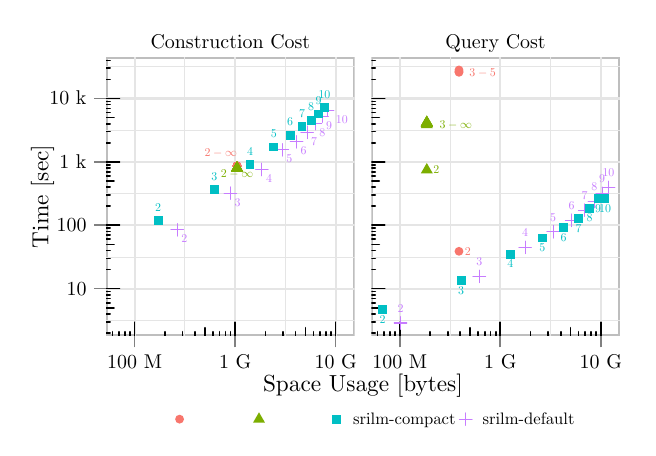
\begin{tikzpicture}[x=1pt,y=1pt]
\definecolor{fillColor}{RGB}{255,255,255}
\path[use as bounding box,fill=fillColor,fill opacity=0.00] (0,0) rectangle (216.81,144.54);
\begin{scope}
\path[clip] (  0.00,  0.00) rectangle (216.81,144.54);
\definecolor{fillColor}{RGB}{255,255,255}

\path[fill=fillColor] (  0.00,  0.00) rectangle (216.81,144.54);
\end{scope}
\begin{scope}
\path[clip] ( 28.36,133.83) rectangle (118.15,144.54);

\path[] ( 28.36,133.83) rectangle (118.15,144.54);
\definecolor{drawColor}{RGB}{0,0,0}

\node[text=drawColor,anchor=base,inner sep=0pt, outer sep=0pt, scale=  0.72] at ( 73.25,136.84) {Construction Cost};
\end{scope}
\begin{scope}
\path[clip] (124.17,133.83) rectangle (213.96,144.54);

\path[] (124.17,133.83) rectangle (213.96,144.54);
\definecolor{drawColor}{RGB}{0,0,0}

\node[text=drawColor,anchor=base,inner sep=0pt, outer sep=0pt, scale=  0.72] at (169.07,136.84) {Query Cost};
\end{scope}
\begin{scope}
\path[clip] ( 28.36, 33.25) rectangle (118.15,133.83);
\definecolor{drawColor}{RGB}{190,190,190}

\path[draw=drawColor,line width= 1.5pt,line join=round,line cap=round] ( 28.36, 33.25) rectangle (118.15,133.83);
\definecolor{drawColor}{gray}{0.90}

\path[draw=drawColor,line width= 0.3pt,line join=round] ( 28.36, 38.79) --
	(118.15, 38.79);

\path[draw=drawColor,line width= 0.3pt,line join=round] ( 28.36, 61.69) --
	(118.15, 61.69);

\path[draw=drawColor,line width= 0.3pt,line join=round] ( 28.36, 84.59) --
	(118.15, 84.59);

\path[draw=drawColor,line width= 0.3pt,line join=round] ( 28.36,107.49) --
	(118.15,107.49);

\path[draw=drawColor,line width= 0.3pt,line join=round] ( 28.36,130.39) --
	(118.15,130.39);

\path[draw=drawColor,line width= 0.3pt,line join=round] ( 56.81, 33.25) --
	( 56.81,133.83);

\path[draw=drawColor,line width= 0.3pt,line join=round] ( 93.13, 33.25) --
	( 93.13,133.83);

\path[draw=drawColor,line width= 0.8pt,line join=round] ( 28.36, 50.24) --
	(118.15, 50.24);

\path[draw=drawColor,line width= 0.8pt,line join=round] ( 28.36, 73.14) --
	(118.15, 73.14);

\path[draw=drawColor,line width= 0.8pt,line join=round] ( 28.36, 96.04) --
	(118.15, 96.04);

\path[draw=drawColor,line width= 0.8pt,line join=round] ( 28.36,118.94) --
	(118.15,118.94);

\path[draw=drawColor,line width= 0.8pt,line join=round] ( 38.65, 33.25) --
	( 38.65,133.83);

\path[draw=drawColor,line width= 0.8pt,line join=round] ( 74.97, 33.25) --
	( 74.97,133.83);

\path[draw=drawColor,line width= 0.8pt,line join=round] (111.29, 33.25) --
	(111.29,133.83);
\definecolor{drawColor}{RGB}{0,0,0}

\path[draw=drawColor,line width= 0.6pt,line join=round,line cap=round] (  2.34, 33.25) -- (  2.34, 38.09);

\path[draw=drawColor,line width= 0.6pt,line join=round,line cap=round] ( 13.27, 33.25) -- ( 13.27, 34.67);

\path[draw=drawColor,line width= 0.6pt,line join=round,line cap=round] ( 19.67, 33.25) -- ( 19.67, 34.67);

\path[draw=drawColor,line width= 0.6pt,line join=round,line cap=round] ( 24.20, 33.25) -- ( 24.20, 34.67);

\path[draw=drawColor,line width= 0.6pt,line join=round,line cap=round] ( 27.72, 33.25) -- ( 27.72, 36.09);

\path[draw=drawColor,line width= 0.6pt,line join=round,line cap=round] ( 30.60, 33.25) -- ( 30.60, 34.67);

\path[draw=drawColor,line width= 0.6pt,line join=round,line cap=round] ( 33.03, 33.25) -- ( 33.03, 34.67);

\path[draw=drawColor,line width= 0.6pt,line join=round,line cap=round] ( 35.14, 33.25) -- ( 35.14, 34.67);

\path[draw=drawColor,line width= 0.6pt,line join=round,line cap=round] ( 36.99, 33.25) -- ( 36.99, 34.67);

\path[draw=drawColor,line width= 0.6pt,line join=round,line cap=round] ( 38.65, 33.25) -- ( 38.65, 38.09);

\path[draw=drawColor,line width= 0.6pt,line join=round,line cap=round] ( 49.59, 33.25) -- ( 49.59, 34.67);

\path[draw=drawColor,line width= 0.6pt,line join=round,line cap=round] ( 55.98, 33.25) -- ( 55.98, 34.67);

\path[draw=drawColor,line width= 0.6pt,line join=round,line cap=round] ( 60.52, 33.25) -- ( 60.52, 34.67);

\path[draw=drawColor,line width= 0.6pt,line join=round,line cap=round] ( 64.04, 33.25) -- ( 64.04, 36.09);

\path[draw=drawColor,line width= 0.6pt,line join=round,line cap=round] ( 66.91, 33.25) -- ( 66.91, 34.67);

\path[draw=drawColor,line width= 0.6pt,line join=round,line cap=round] ( 69.34, 33.25) -- ( 69.34, 34.67);

\path[draw=drawColor,line width= 0.6pt,line join=round,line cap=round] ( 71.45, 33.25) -- ( 71.45, 34.67);

\path[draw=drawColor,line width= 0.6pt,line join=round,line cap=round] ( 73.31, 33.25) -- ( 73.31, 34.67);

\path[draw=drawColor,line width= 0.6pt,line join=round,line cap=round] ( 74.97, 33.25) -- ( 74.97, 38.09);

\path[draw=drawColor,line width= 0.6pt,line join=round,line cap=round] ( 85.90, 33.25) -- ( 85.90, 34.67);

\path[draw=drawColor,line width= 0.6pt,line join=round,line cap=round] ( 92.30, 33.25) -- ( 92.30, 34.67);

\path[draw=drawColor,line width= 0.6pt,line join=round,line cap=round] ( 96.83, 33.25) -- ( 96.83, 34.67);

\path[draw=drawColor,line width= 0.6pt,line join=round,line cap=round] (100.35, 33.25) -- (100.35, 36.09);

\path[draw=drawColor,line width= 0.6pt,line join=round,line cap=round] (103.23, 33.25) -- (103.23, 34.67);

\path[draw=drawColor,line width= 0.6pt,line join=round,line cap=round] (105.66, 33.25) -- (105.66, 34.67);

\path[draw=drawColor,line width= 0.6pt,line join=round,line cap=round] (107.77, 33.25) -- (107.77, 34.67);

\path[draw=drawColor,line width= 0.6pt,line join=round,line cap=round] (109.62, 33.25) -- (109.62, 34.67);

\path[draw=drawColor,line width= 0.6pt,line join=round,line cap=round] (111.29, 33.25) -- (111.29, 38.09);

\path[draw=drawColor,line width= 0.6pt,line join=round,line cap=round] (122.22, 33.25) -- (122.22, 34.67);

\path[draw=drawColor,line width= 0.6pt,line join=round,line cap=round] (128.61, 33.25) -- (128.61, 34.67);

\path[draw=drawColor,line width= 0.6pt,line join=round,line cap=round] (133.15, 33.25) -- (133.15, 34.67);

\path[draw=drawColor,line width= 0.6pt,line join=round,line cap=round] (136.67, 33.25) -- (136.67, 36.09);

\path[draw=drawColor,line width= 0.6pt,line join=round,line cap=round] (139.54, 33.25) -- (139.54, 34.67);

\path[draw=drawColor,line width= 0.6pt,line join=round,line cap=round] (141.98, 33.25) -- (141.98, 34.67);

\path[draw=drawColor,line width= 0.6pt,line join=round,line cap=round] (144.08, 33.25) -- (144.08, 34.67);

\path[draw=drawColor,line width= 0.6pt,line join=round,line cap=round] (145.94, 33.25) -- (145.94, 34.67);

\path[draw=drawColor,line width= 0.6pt,line join=round,line cap=round] (147.60, 33.25) -- (147.60, 38.09);

\path[draw=drawColor,line width= 0.6pt,line join=round,line cap=round] ( 28.36, 27.34) -- ( 33.20, 27.34);

\path[draw=drawColor,line width= 0.6pt,line join=round,line cap=round] ( 28.36, 34.23) -- ( 29.78, 34.23);

\path[draw=drawColor,line width= 0.6pt,line join=round,line cap=round] ( 28.36, 38.26) -- ( 29.78, 38.26);

\path[draw=drawColor,line width= 0.6pt,line join=round,line cap=round] ( 28.36, 41.12) -- ( 29.78, 41.12);

\path[draw=drawColor,line width= 0.6pt,line join=round,line cap=round] ( 28.36, 43.34) -- ( 31.20, 43.34);

\path[draw=drawColor,line width= 0.6pt,line join=round,line cap=round] ( 28.36, 45.16) -- ( 29.78, 45.16);

\path[draw=drawColor,line width= 0.6pt,line join=round,line cap=round] ( 28.36, 46.69) -- ( 29.78, 46.69);

\path[draw=drawColor,line width= 0.6pt,line join=round,line cap=round] ( 28.36, 48.02) -- ( 29.78, 48.02);

\path[draw=drawColor,line width= 0.6pt,line join=round,line cap=round] ( 28.36, 49.19) -- ( 29.78, 49.19);

\path[draw=drawColor,line width= 0.6pt,line join=round,line cap=round] ( 28.36, 50.24) -- ( 33.20, 50.24);

\path[draw=drawColor,line width= 0.6pt,line join=round,line cap=round] ( 28.36, 57.13) -- ( 29.78, 57.13);

\path[draw=drawColor,line width= 0.6pt,line join=round,line cap=round] ( 28.36, 61.16) -- ( 29.78, 61.16);

\path[draw=drawColor,line width= 0.6pt,line join=round,line cap=round] ( 28.36, 64.02) -- ( 29.78, 64.02);

\path[draw=drawColor,line width= 0.6pt,line join=round,line cap=round] ( 28.36, 66.24) -- ( 31.20, 66.24);

\path[draw=drawColor,line width= 0.6pt,line join=round,line cap=round] ( 28.36, 68.06) -- ( 29.78, 68.06);

\path[draw=drawColor,line width= 0.6pt,line join=round,line cap=round] ( 28.36, 69.59) -- ( 29.78, 69.59);

\path[draw=drawColor,line width= 0.6pt,line join=round,line cap=round] ( 28.36, 70.92) -- ( 29.78, 70.92);

\path[draw=drawColor,line width= 0.6pt,line join=round,line cap=round] ( 28.36, 72.09) -- ( 29.78, 72.09);

\path[draw=drawColor,line width= 0.6pt,line join=round,line cap=round] ( 28.36, 73.14) -- ( 33.20, 73.14);

\path[draw=drawColor,line width= 0.6pt,line join=round,line cap=round] ( 28.36, 80.03) -- ( 29.78, 80.03);

\path[draw=drawColor,line width= 0.6pt,line join=round,line cap=round] ( 28.36, 84.07) -- ( 29.78, 84.07);

\path[draw=drawColor,line width= 0.6pt,line join=round,line cap=round] ( 28.36, 86.93) -- ( 29.78, 86.93);

\path[draw=drawColor,line width= 0.6pt,line join=round,line cap=round] ( 28.36, 89.15) -- ( 31.20, 89.15);

\path[draw=drawColor,line width= 0.6pt,line join=round,line cap=round] ( 28.36, 90.96) -- ( 29.78, 90.96);

\path[draw=drawColor,line width= 0.6pt,line join=round,line cap=round] ( 28.36, 92.49) -- ( 29.78, 92.49);

\path[draw=drawColor,line width= 0.6pt,line join=round,line cap=round] ( 28.36, 93.82) -- ( 29.78, 93.82);

\path[draw=drawColor,line width= 0.6pt,line join=round,line cap=round] ( 28.36, 94.99) -- ( 29.78, 94.99);

\path[draw=drawColor,line width= 0.6pt,line join=round,line cap=round] ( 28.36, 96.04) -- ( 33.20, 96.04);

\path[draw=drawColor,line width= 0.6pt,line join=round,line cap=round] ( 28.36,102.93) -- ( 29.78,102.93);

\path[draw=drawColor,line width= 0.6pt,line join=round,line cap=round] ( 28.36,106.97) -- ( 29.78,106.97);

\path[draw=drawColor,line width= 0.6pt,line join=round,line cap=round] ( 28.36,109.83) -- ( 29.78,109.83);

\path[draw=drawColor,line width= 0.6pt,line join=round,line cap=round] ( 28.36,112.05) -- ( 31.20,112.05);

\path[draw=drawColor,line width= 0.6pt,line join=round,line cap=round] ( 28.36,113.86) -- ( 29.78,113.86);

\path[draw=drawColor,line width= 0.6pt,line join=round,line cap=round] ( 28.36,115.39) -- ( 29.78,115.39);

\path[draw=drawColor,line width= 0.6pt,line join=round,line cap=round] ( 28.36,116.72) -- ( 29.78,116.72);

\path[draw=drawColor,line width= 0.6pt,line join=round,line cap=round] ( 28.36,117.89) -- ( 29.78,117.89);

\path[draw=drawColor,line width= 0.6pt,line join=round,line cap=round] ( 28.36,118.94) -- ( 33.20,118.94);

\path[draw=drawColor,line width= 0.6pt,line join=round,line cap=round] ( 28.36,125.84) -- ( 29.78,125.84);

\path[draw=drawColor,line width= 0.6pt,line join=round,line cap=round] ( 28.36,129.87) -- ( 29.78,129.87);

\path[draw=drawColor,line width= 0.6pt,line join=round,line cap=round] ( 28.36,132.73) -- ( 29.78,132.73);

\path[draw=drawColor,line width= 0.6pt,line join=round,line cap=round] ( 28.36,134.95) -- ( 31.20,134.95);

\path[draw=drawColor,line width= 0.6pt,line join=round,line cap=round] ( 28.36,136.76) -- ( 29.78,136.76);

\path[draw=drawColor,line width= 0.6pt,line join=round,line cap=round] ( 28.36,138.30) -- ( 29.78,138.30);

\path[draw=drawColor,line width= 0.6pt,line join=round,line cap=round] ( 28.36,139.62) -- ( 29.78,139.62);

\path[draw=drawColor,line width= 0.6pt,line join=round,line cap=round] ( 28.36,140.80) -- ( 29.78,140.80);

\path[draw=drawColor,line width= 0.6pt,line join=round,line cap=round] ( 28.36,141.84) -- ( 33.20,141.84);
\definecolor{drawColor}{RGB}{199,124,255}

\path[draw=drawColor,line width= 0.4pt,line join=round,line cap=round] ( 51.78, 71.49) -- ( 56.30, 71.49);

\path[draw=drawColor,line width= 0.4pt,line join=round,line cap=round] ( 54.04, 69.23) -- ( 54.04, 73.75);

\path[draw=drawColor,line width= 0.4pt,line join=round,line cap=round] ( 71.01, 84.73) -- ( 75.53, 84.73);

\path[draw=drawColor,line width= 0.4pt,line join=round,line cap=round] ( 73.27, 82.47) -- ( 73.27, 86.99);

\path[draw=drawColor,line width= 0.4pt,line join=round,line cap=round] ( 82.38, 93.31) -- ( 86.91, 93.31);

\path[draw=drawColor,line width= 0.4pt,line join=round,line cap=round] ( 84.65, 91.04) -- ( 84.65, 95.57);

\path[draw=drawColor,line width= 0.4pt,line join=round,line cap=round] ( 89.76,100.37) -- ( 94.28,100.37);

\path[draw=drawColor,line width= 0.4pt,line join=round,line cap=round] ( 92.02, 98.11) -- ( 92.02,102.64);

\path[draw=drawColor,line width= 0.4pt,line join=round,line cap=round] ( 94.89,103.29) -- ( 99.41,103.29);

\path[draw=drawColor,line width= 0.4pt,line join=round,line cap=round] ( 97.15,101.03) -- ( 97.15,105.55);

\path[draw=drawColor,line width= 0.4pt,line join=round,line cap=round] ( 98.71,106.75) -- (103.24,106.75);

\path[draw=drawColor,line width= 0.4pt,line join=round,line cap=round] (100.98,104.49) -- (100.98,109.01);

\path[draw=drawColor,line width= 0.4pt,line join=round,line cap=round] (101.70,109.84) -- (106.23,109.84);

\path[draw=drawColor,line width= 0.4pt,line join=round,line cap=round] (103.96,107.58) -- (103.96,112.10);

\path[draw=drawColor,line width= 0.4pt,line join=round,line cap=round] (104.12,112.58) -- (108.64,112.58);

\path[draw=drawColor,line width= 0.4pt,line join=round,line cap=round] (106.38,110.32) -- (106.38,114.85);

\path[draw=drawColor,line width= 0.4pt,line join=round,line cap=round] (106.12,114.77) -- (110.65,114.77);

\path[draw=drawColor,line width= 0.4pt,line join=round,line cap=round] (108.38,112.51) -- (108.38,117.04);
\definecolor{fillColor}{RGB}{0,191,196}

\path[fill=fillColor] ( 45.55, 73.26) --
	( 48.75, 73.26) --
	( 48.75, 76.46) --
	( 45.55, 76.46) --
	cycle;

\path[fill=fillColor] ( 65.83, 84.45) --
	( 69.03, 84.45) --
	( 69.03, 87.65) --
	( 65.83, 87.65) --
	cycle;

\path[fill=fillColor] ( 78.75, 93.45) --
	( 81.96, 93.45) --
	( 81.96, 96.65) --
	( 78.75, 96.65) --
	cycle;

\path[fill=fillColor] ( 87.33, 99.84) --
	( 90.53, 99.84) --
	( 90.53,103.04) --
	( 87.33,103.04) --
	cycle;

\path[fill=fillColor] ( 93.24,104.12) --
	( 96.44,104.12) --
	( 96.44,107.33) --
	( 93.24,107.33) --
	cycle;

\path[fill=fillColor] ( 97.55,107.25) --
	(100.75,107.25) --
	(100.75,110.45) --
	( 97.55,110.45) --
	cycle;

\path[fill=fillColor] (100.86,109.53) --
	(104.06,109.53) --
	(104.06,112.74) --
	(100.86,112.74) --
	cycle;

\path[fill=fillColor] (103.49,111.77) --
	(106.69,111.77) --
	(106.69,114.97) --
	(103.49,114.97) --
	cycle;

\path[fill=fillColor] (105.65,114.08) --
	(108.85,114.08) --
	(108.85,117.28) --
	(105.65,117.28) --
	cycle;
\definecolor{fillColor}{RGB}{248,118,109}

\path[fill=fillColor] ( 75.65, 94.55) circle (  1.60);

\path[fill=fillColor] ( 75.65, 94.55) circle (  1.60);

\path[fill=fillColor] ( 75.65, 94.55) circle (  1.60);

\path[fill=fillColor] ( 75.65, 94.55) circle (  1.60);

\path[fill=fillColor] ( 75.65, 94.55) circle (  1.60);

\path[fill=fillColor] ( 75.65, 94.55) circle (  1.60);

\path[fill=fillColor] ( 75.65, 94.55) circle (  1.60);

\path[fill=fillColor] ( 75.65, 94.55) circle (  1.60);

\path[fill=fillColor] ( 75.65, 94.55) circle (  1.60);
\definecolor{fillColor}{RGB}{124,174,0}

\path[fill=fillColor] ( 75.65, 96.27) --
	( 77.81, 92.54) --
	( 73.50, 92.54) --
	cycle;

\path[fill=fillColor] ( 75.65, 96.27) --
	( 77.81, 92.54) --
	( 73.50, 92.54) --
	cycle;

\path[fill=fillColor] ( 75.65, 96.27) --
	( 77.81, 92.54) --
	( 73.50, 92.54) --
	cycle;

\path[fill=fillColor] ( 75.65, 96.27) --
	( 77.81, 92.54) --
	( 73.50, 92.54) --
	cycle;

\path[fill=fillColor] ( 75.65, 96.27) --
	( 77.81, 92.54) --
	( 73.50, 92.54) --
	cycle;

\path[fill=fillColor] ( 75.65, 96.27) --
	( 77.81, 92.54) --
	( 73.50, 92.54) --
	cycle;

\path[fill=fillColor] ( 75.65, 96.27) --
	( 77.81, 92.54) --
	( 73.50, 92.54) --
	cycle;

\path[fill=fillColor] ( 75.65, 96.27) --
	( 77.81, 92.54) --
	( 73.50, 92.54) --
	cycle;

\path[fill=fillColor] ( 75.65, 96.27) --
	( 77.81, 92.54) --
	( 73.50, 92.54) --
	cycle;

\node[text=drawColor,anchor=base west,inner sep=0pt, outer sep=0pt, scale=  0.43] at ( 55.53, 66.78) {2};

\node[text=drawColor,anchor=base west,inner sep=0pt, outer sep=0pt, scale=  0.43] at ( 74.76, 80.02) {3};

\node[text=drawColor,anchor=base west,inner sep=0pt, outer sep=0pt, scale=  0.43] at ( 86.13, 88.60) {4};

\node[text=drawColor,anchor=base west,inner sep=0pt, outer sep=0pt, scale=  0.43] at ( 93.51, 95.67) {5};

\node[text=drawColor,anchor=base west,inner sep=0pt, outer sep=0pt, scale=  0.43] at ( 98.64, 98.58) {6};

\node[text=drawColor,anchor=base west,inner sep=0pt, outer sep=0pt, scale=  0.43] at (102.46,102.04) {7};

\node[text=drawColor,anchor=base west,inner sep=0pt, outer sep=0pt, scale=  0.43] at (105.45,105.14) {8};

\node[text=drawColor,anchor=base west,inner sep=0pt, outer sep=0pt, scale=  0.43] at (107.87,107.88) {9};

\node[text=drawColor,anchor=base west,inner sep=0pt, outer sep=0pt, scale=  0.43] at (111.36,110.07) {10};
\definecolor{drawColor}{RGB}{0,191,196}

\node[text=drawColor,anchor=base,inner sep=0pt, outer sep=0pt, scale=  0.43] at ( 47.15, 78.18) {2};

\node[text=drawColor,anchor=base,inner sep=0pt, outer sep=0pt, scale=  0.43] at ( 67.43, 89.38) {3};

\node[text=drawColor,anchor=base,inner sep=0pt, outer sep=0pt, scale=  0.43] at ( 80.35, 98.37) {4};

\node[text=drawColor,anchor=base,inner sep=0pt, outer sep=0pt, scale=  0.43] at ( 88.93,104.76) {5};

\node[text=drawColor,anchor=base,inner sep=0pt, outer sep=0pt, scale=  0.43] at ( 94.84,109.05) {6};

\node[text=drawColor,anchor=base,inner sep=0pt, outer sep=0pt, scale=  0.43] at ( 99.15,112.17) {7};

\node[text=drawColor,anchor=base,inner sep=0pt, outer sep=0pt, scale=  0.43] at (102.46,114.46) {8};

\node[text=drawColor,anchor=base,inner sep=0pt, outer sep=0pt, scale=  0.43] at (105.09,116.69) {9};

\node[text=drawColor,anchor=base,inner sep=0pt, outer sep=0pt, scale=  0.43] at (107.25,119.00) {10};
\definecolor{drawColor}{RGB}{248,118,109}

\node[text=drawColor,anchor=base east,inner sep=0pt, outer sep=0pt, scale=  0.43] at ( 75.65, 97.87) {$2-\\\infty$};
\definecolor{drawColor}{RGB}{124,174,0}

\node[text=drawColor,anchor=base,inner sep=0pt, outer sep=0pt, scale=  0.43] at ( 75.65, 90.46) {$2-\\\infty$};
\end{scope}
\begin{scope}
\path[clip] (124.17, 33.25) rectangle (213.96,133.83);
\definecolor{drawColor}{RGB}{190,190,190}

\path[draw=drawColor,line width= 1.5pt,line join=round,line cap=round] (124.17, 33.25) rectangle (213.96,133.83);
\definecolor{drawColor}{gray}{0.90}

\path[draw=drawColor,line width= 0.3pt,line join=round] (124.17, 38.79) --
	(213.96, 38.79);

\path[draw=drawColor,line width= 0.3pt,line join=round] (124.17, 61.69) --
	(213.96, 61.69);

\path[draw=drawColor,line width= 0.3pt,line join=round] (124.17, 84.59) --
	(213.96, 84.59);

\path[draw=drawColor,line width= 0.3pt,line join=round] (124.17,107.49) --
	(213.96,107.49);

\path[draw=drawColor,line width= 0.3pt,line join=round] (124.17,130.39) --
	(213.96,130.39);

\path[draw=drawColor,line width= 0.3pt,line join=round] (152.63, 33.25) --
	(152.63,133.83);

\path[draw=drawColor,line width= 0.3pt,line join=round] (188.94, 33.25) --
	(188.94,133.83);

\path[draw=drawColor,line width= 0.8pt,line join=round] (124.17, 50.24) --
	(213.96, 50.24);

\path[draw=drawColor,line width= 0.8pt,line join=round] (124.17, 73.14) --
	(213.96, 73.14);

\path[draw=drawColor,line width= 0.8pt,line join=round] (124.17, 96.04) --
	(213.96, 96.04);

\path[draw=drawColor,line width= 0.8pt,line join=round] (124.17,118.94) --
	(213.96,118.94);

\path[draw=drawColor,line width= 0.8pt,line join=round] (134.47, 33.25) --
	(134.47,133.83);

\path[draw=drawColor,line width= 0.8pt,line join=round] (170.78, 33.25) --
	(170.78,133.83);

\path[draw=drawColor,line width= 0.8pt,line join=round] (207.10, 33.25) --
	(207.10,133.83);
\definecolor{drawColor}{RGB}{0,0,0}

\path[draw=drawColor,line width= 0.6pt,line join=round,line cap=round] ( 98.15, 33.25) -- ( 98.15, 38.09);

\path[draw=drawColor,line width= 0.6pt,line join=round,line cap=round] (109.09, 33.25) -- (109.09, 34.67);

\path[draw=drawColor,line width= 0.6pt,line join=round,line cap=round] (115.48, 33.25) -- (115.48, 34.67);

\path[draw=drawColor,line width= 0.6pt,line join=round,line cap=round] (120.02, 33.25) -- (120.02, 34.67);

\path[draw=drawColor,line width= 0.6pt,line join=round,line cap=round] (123.54, 33.25) -- (123.54, 36.09);

\path[draw=drawColor,line width= 0.6pt,line join=round,line cap=round] (126.41, 33.25) -- (126.41, 34.67);

\path[draw=drawColor,line width= 0.6pt,line join=round,line cap=round] (128.84, 33.25) -- (128.84, 34.67);

\path[draw=drawColor,line width= 0.6pt,line join=round,line cap=round] (130.95, 33.25) -- (130.95, 34.67);

\path[draw=drawColor,line width= 0.6pt,line join=round,line cap=round] (132.81, 33.25) -- (132.81, 34.67);

\path[draw=drawColor,line width= 0.6pt,line join=round,line cap=round] (134.47, 33.25) -- (134.47, 38.09);

\path[draw=drawColor,line width= 0.6pt,line join=round,line cap=round] (145.40, 33.25) -- (145.40, 34.67);

\path[draw=drawColor,line width= 0.6pt,line join=round,line cap=round] (151.80, 33.25) -- (151.80, 34.67);

\path[draw=drawColor,line width= 0.6pt,line join=round,line cap=round] (156.33, 33.25) -- (156.33, 34.67);

\path[draw=drawColor,line width= 0.6pt,line join=round,line cap=round] (159.85, 33.25) -- (159.85, 36.09);

\path[draw=drawColor,line width= 0.6pt,line join=round,line cap=round] (162.73, 33.25) -- (162.73, 34.67);

\path[draw=drawColor,line width= 0.6pt,line join=round,line cap=round] (165.16, 33.25) -- (165.16, 34.67);

\path[draw=drawColor,line width= 0.6pt,line join=round,line cap=round] (167.26, 33.25) -- (167.26, 34.67);

\path[draw=drawColor,line width= 0.6pt,line join=round,line cap=round] (169.12, 33.25) -- (169.12, 34.67);

\path[draw=drawColor,line width= 0.6pt,line join=round,line cap=round] (170.78, 33.25) -- (170.78, 38.09);

\path[draw=drawColor,line width= 0.6pt,line join=round,line cap=round] (181.72, 33.25) -- (181.72, 34.67);

\path[draw=drawColor,line width= 0.6pt,line join=round,line cap=round] (188.11, 33.25) -- (188.11, 34.67);

\path[draw=drawColor,line width= 0.6pt,line join=round,line cap=round] (192.65, 33.25) -- (192.65, 34.67);

\path[draw=drawColor,line width= 0.6pt,line join=round,line cap=round] (196.17, 33.25) -- (196.17, 36.09);

\path[draw=drawColor,line width= 0.6pt,line join=round,line cap=round] (199.04, 33.25) -- (199.04, 34.67);

\path[draw=drawColor,line width= 0.6pt,line join=round,line cap=round] (201.47, 33.25) -- (201.47, 34.67);

\path[draw=drawColor,line width= 0.6pt,line join=round,line cap=round] (203.58, 33.25) -- (203.58, 34.67);

\path[draw=drawColor,line width= 0.6pt,line join=round,line cap=round] (205.44, 33.25) -- (205.44, 34.67);

\path[draw=drawColor,line width= 0.6pt,line join=round,line cap=round] (207.10, 33.25) -- (207.10, 38.09);

\path[draw=drawColor,line width= 0.6pt,line join=round,line cap=round] (124.17, 27.34) -- (129.01, 27.34);

\path[draw=drawColor,line width= 0.6pt,line join=round,line cap=round] (124.17, 34.23) -- (125.60, 34.23);

\path[draw=drawColor,line width= 0.6pt,line join=round,line cap=round] (124.17, 38.26) -- (125.60, 38.26);

\path[draw=drawColor,line width= 0.6pt,line join=round,line cap=round] (124.17, 41.12) -- (125.60, 41.12);

\path[draw=drawColor,line width= 0.6pt,line join=round,line cap=round] (124.17, 43.34) -- (127.02, 43.34);

\path[draw=drawColor,line width= 0.6pt,line join=round,line cap=round] (124.17, 45.16) -- (125.60, 45.16);

\path[draw=drawColor,line width= 0.6pt,line join=round,line cap=round] (124.17, 46.69) -- (125.60, 46.69);

\path[draw=drawColor,line width= 0.6pt,line join=round,line cap=round] (124.17, 48.02) -- (125.60, 48.02);

\path[draw=drawColor,line width= 0.6pt,line join=round,line cap=round] (124.17, 49.19) -- (125.60, 49.19);

\path[draw=drawColor,line width= 0.6pt,line join=round,line cap=round] (124.17, 50.24) -- (129.01, 50.24);

\path[draw=drawColor,line width= 0.6pt,line join=round,line cap=round] (124.17, 57.13) -- (125.60, 57.13);

\path[draw=drawColor,line width= 0.6pt,line join=round,line cap=round] (124.17, 61.16) -- (125.60, 61.16);

\path[draw=drawColor,line width= 0.6pt,line join=round,line cap=round] (124.17, 64.02) -- (125.60, 64.02);

\path[draw=drawColor,line width= 0.6pt,line join=round,line cap=round] (124.17, 66.24) -- (127.02, 66.24);

\path[draw=drawColor,line width= 0.6pt,line join=round,line cap=round] (124.17, 68.06) -- (125.60, 68.06);

\path[draw=drawColor,line width= 0.6pt,line join=round,line cap=round] (124.17, 69.59) -- (125.60, 69.59);

\path[draw=drawColor,line width= 0.6pt,line join=round,line cap=round] (124.17, 70.92) -- (125.60, 70.92);

\path[draw=drawColor,line width= 0.6pt,line join=round,line cap=round] (124.17, 72.09) -- (125.60, 72.09);

\path[draw=drawColor,line width= 0.6pt,line join=round,line cap=round] (124.17, 73.14) -- (129.01, 73.14);

\path[draw=drawColor,line width= 0.6pt,line join=round,line cap=round] (124.17, 80.03) -- (125.60, 80.03);

\path[draw=drawColor,line width= 0.6pt,line join=round,line cap=round] (124.17, 84.07) -- (125.60, 84.07);

\path[draw=drawColor,line width= 0.6pt,line join=round,line cap=round] (124.17, 86.93) -- (125.60, 86.93);

\path[draw=drawColor,line width= 0.6pt,line join=round,line cap=round] (124.17, 89.15) -- (127.02, 89.15);

\path[draw=drawColor,line width= 0.6pt,line join=round,line cap=round] (124.17, 90.96) -- (125.60, 90.96);

\path[draw=drawColor,line width= 0.6pt,line join=round,line cap=round] (124.17, 92.49) -- (125.60, 92.49);

\path[draw=drawColor,line width= 0.6pt,line join=round,line cap=round] (124.17, 93.82) -- (125.60, 93.82);

\path[draw=drawColor,line width= 0.6pt,line join=round,line cap=round] (124.17, 94.99) -- (125.60, 94.99);

\path[draw=drawColor,line width= 0.6pt,line join=round,line cap=round] (124.17, 96.04) -- (129.01, 96.04);

\path[draw=drawColor,line width= 0.6pt,line join=round,line cap=round] (124.17,102.93) -- (125.60,102.93);

\path[draw=drawColor,line width= 0.6pt,line join=round,line cap=round] (124.17,106.97) -- (125.60,106.97);

\path[draw=drawColor,line width= 0.6pt,line join=round,line cap=round] (124.17,109.83) -- (125.60,109.83);

\path[draw=drawColor,line width= 0.6pt,line join=round,line cap=round] (124.17,112.05) -- (127.02,112.05);

\path[draw=drawColor,line width= 0.6pt,line join=round,line cap=round] (124.17,113.86) -- (125.60,113.86);

\path[draw=drawColor,line width= 0.6pt,line join=round,line cap=round] (124.17,115.39) -- (125.60,115.39);

\path[draw=drawColor,line width= 0.6pt,line join=round,line cap=round] (124.17,116.72) -- (125.60,116.72);

\path[draw=drawColor,line width= 0.6pt,line join=round,line cap=round] (124.17,117.89) -- (125.60,117.89);

\path[draw=drawColor,line width= 0.6pt,line join=round,line cap=round] (124.17,118.94) -- (129.01,118.94);

\path[draw=drawColor,line width= 0.6pt,line join=round,line cap=round] (124.17,125.84) -- (125.60,125.84);

\path[draw=drawColor,line width= 0.6pt,line join=round,line cap=round] (124.17,129.87) -- (125.60,129.87);

\path[draw=drawColor,line width= 0.6pt,line join=round,line cap=round] (124.17,132.73) -- (125.60,132.73);

\path[draw=drawColor,line width= 0.6pt,line join=round,line cap=round] (124.17,134.95) -- (127.02,134.95);

\path[draw=drawColor,line width= 0.6pt,line join=round,line cap=round] (124.17,136.76) -- (125.60,136.76);

\path[draw=drawColor,line width= 0.6pt,line join=round,line cap=round] (124.17,138.30) -- (125.60,138.30);

\path[draw=drawColor,line width= 0.6pt,line join=round,line cap=round] (124.17,139.62) -- (125.60,139.62);

\path[draw=drawColor,line width= 0.6pt,line join=round,line cap=round] (124.17,140.80) -- (125.60,140.80);

\path[draw=drawColor,line width= 0.6pt,line join=round,line cap=round] (124.17,141.84) -- (129.01,141.84);
\definecolor{drawColor}{RGB}{199,124,255}

\path[draw=drawColor,line width= 0.4pt,line join=round,line cap=round] (132.47, 37.82) -- (136.99, 37.82);

\path[draw=drawColor,line width= 0.4pt,line join=round,line cap=round] (134.73, 35.56) -- (134.73, 40.08);

\path[draw=drawColor,line width= 0.4pt,line join=round,line cap=round] (160.92, 54.66) -- (165.45, 54.66);

\path[draw=drawColor,line width= 0.4pt,line join=round,line cap=round] (163.18, 52.40) -- (163.18, 56.92);

\path[draw=drawColor,line width= 0.4pt,line join=round,line cap=round] (177.49, 65.14) -- (182.01, 65.14);

\path[draw=drawColor,line width= 0.4pt,line join=round,line cap=round] (179.75, 62.88) -- (179.75, 67.41);

\path[draw=drawColor,line width= 0.4pt,line join=round,line cap=round] (187.63, 70.80) -- (192.15, 70.80);

\path[draw=drawColor,line width= 0.4pt,line join=round,line cap=round] (189.89, 68.53) -- (189.89, 73.06);

\path[draw=drawColor,line width= 0.4pt,line join=round,line cap=round] (194.27, 74.94) -- (198.80, 74.94);

\path[draw=drawColor,line width= 0.4pt,line join=round,line cap=round] (196.54, 72.67) -- (196.54, 77.20);

\path[draw=drawColor,line width= 0.4pt,line join=round,line cap=round] (198.98, 78.59) -- (203.51, 78.59);

\path[draw=drawColor,line width= 0.4pt,line join=round,line cap=round] (201.24, 76.33) -- (201.24, 80.85);

\path[draw=drawColor,line width= 0.4pt,line join=round,line cap=round] (202.53, 81.70) -- (207.06, 81.70);

\path[draw=drawColor,line width= 0.4pt,line join=round,line cap=round] (204.80, 79.44) -- (204.80, 83.96);

\path[draw=drawColor,line width= 0.4pt,line join=round,line cap=round] (205.34, 84.67) -- (209.86, 84.67);

\path[draw=drawColor,line width= 0.4pt,line join=round,line cap=round] (207.60, 82.40) -- (207.60, 86.93);

\path[draw=drawColor,line width= 0.4pt,line join=round,line cap=round] (207.62, 86.78) -- (212.15, 86.78);

\path[draw=drawColor,line width= 0.4pt,line join=round,line cap=round] (209.88, 84.52) -- (209.88, 89.04);
\definecolor{fillColor}{RGB}{0,191,196}

\path[fill=fillColor] (126.65, 41.06) --
	(129.85, 41.06) --
	(129.85, 44.26) --
	(126.65, 44.26) --
	cycle;

\path[fill=fillColor] (155.05, 51.52) --
	(158.25, 51.52) --
	(158.25, 54.72) --
	(155.05, 54.72) --
	cycle;

\path[fill=fillColor] (172.79, 61.12) --
	(175.99, 61.12) --
	(175.99, 64.32) --
	(172.79, 64.32) --
	cycle;

\path[fill=fillColor] (184.34, 66.93) --
	(187.54, 66.93) --
	(187.54, 70.13) --
	(184.34, 70.13) --
	cycle;

\path[fill=fillColor] (192.06, 70.71) --
	(195.26, 70.71) --
	(195.26, 73.91) --
	(192.06, 73.91) --
	cycle;

\path[fill=fillColor] (197.46, 73.83) --
	(200.66, 73.83) --
	(200.66, 77.03) --
	(197.46, 77.03) --
	cycle;

\path[fill=fillColor] (201.45, 77.75) --
	(204.65, 77.75) --
	(204.65, 80.95) --
	(201.45, 80.95) --
	cycle;

\path[fill=fillColor] (204.55, 81.21) --
	(207.75, 81.21) --
	(207.75, 84.41) --
	(204.55, 84.41) --
	cycle;

\path[fill=fillColor] (207.03, 81.07) --
	(210.23, 81.07) --
	(210.23, 84.27) --
	(207.03, 84.27) --
	cycle;
\definecolor{fillColor}{RGB}{248,118,109}

\path[fill=fillColor] (155.85, 63.73) circle (  1.60);

\path[fill=fillColor] (155.85,128.41) circle (  1.60);

\path[fill=fillColor] (155.85,128.63) circle (  1.60);

\path[fill=fillColor] (155.85,129.26) circle (  1.60);
\definecolor{fillColor}{RGB}{124,174,0}

\path[fill=fillColor] (144.22, 95.64) --
	(146.38, 91.91) --
	(142.07, 91.91) --
	cycle;

\path[fill=fillColor] (144.22,111.98) --
	(146.38,108.25) --
	(142.07,108.25) --
	cycle;

\path[fill=fillColor] (144.22,112.64) --
	(146.38,108.91) --
	(142.07,108.91) --
	cycle;

\path[fill=fillColor] (144.22,112.42) --
	(146.38,108.69) --
	(142.07,108.69) --
	cycle;

\path[fill=fillColor] (144.22,112.47) --
	(146.38,108.73) --
	(142.07,108.73) --
	cycle;

\path[fill=fillColor] (144.22,112.80) --
	(146.38,109.06) --
	(142.07,109.06) --
	cycle;

\path[fill=fillColor] (144.22,112.63) --
	(146.38,108.90) --
	(142.07,108.90) --
	cycle;

\path[fill=fillColor] (144.22,112.83) --
	(146.38,109.09) --
	(142.07,109.09) --
	cycle;

\path[fill=fillColor] (144.22,112.59) --
	(146.38,108.85) --
	(142.07,108.85) --
	cycle;
\definecolor{drawColor}{RGB}{248,118,109}

\node[text=drawColor,anchor=base west,inner sep=0pt, outer sep=0pt, scale=  0.43] at (157.98, 62.35) {$2$};

\node[text=drawColor,anchor=base west,inner sep=0pt, outer sep=0pt, scale=  0.43] at (159.63,127.03) {$3-5$};
\definecolor{drawColor}{RGB}{124,174,0}

\node[text=drawColor,anchor=base west,inner sep=0pt, outer sep=0pt, scale=  0.43] at (146.56, 91.77) {$2$};

\node[text=drawColor,anchor=base west,inner sep=0pt, outer sep=0pt, scale=  0.43] at (148.85,108.11) {$3-\\\infty$};
\definecolor{drawColor}{RGB}{199,124,255}

\node[text=drawColor,anchor=base,inner sep=0pt, outer sep=0pt, scale=  0.43] at (134.73, 41.70) {2};

\node[text=drawColor,anchor=base,inner sep=0pt, outer sep=0pt, scale=  0.43] at (163.18, 58.53) {3};

\node[text=drawColor,anchor=base,inner sep=0pt, outer sep=0pt, scale=  0.43] at (179.75, 69.02) {4};

\node[text=drawColor,anchor=base,inner sep=0pt, outer sep=0pt, scale=  0.43] at (189.89, 74.67) {5};

\node[text=drawColor,anchor=base,inner sep=0pt, outer sep=0pt, scale=  0.43] at (196.54, 78.81) {6};

\node[text=drawColor,anchor=base,inner sep=0pt, outer sep=0pt, scale=  0.43] at (201.24, 82.47) {7};

\node[text=drawColor,anchor=base,inner sep=0pt, outer sep=0pt, scale=  0.43] at (204.80, 85.57) {8};

\node[text=drawColor,anchor=base,inner sep=0pt, outer sep=0pt, scale=  0.43] at (207.60, 88.54) {9};

\node[text=drawColor,anchor=base,inner sep=0pt, outer sep=0pt, scale=  0.43] at (209.88, 90.66) {10};
\definecolor{drawColor}{RGB}{0,191,196}

\node[text=drawColor,anchor=base,inner sep=0pt, outer sep=0pt, scale=  0.43] at (128.25, 37.68) {2};

\node[text=drawColor,anchor=base,inner sep=0pt, outer sep=0pt, scale=  0.43] at (156.65, 48.13) {3};

\node[text=drawColor,anchor=base,inner sep=0pt, outer sep=0pt, scale=  0.43] at (174.39, 57.73) {4};

\node[text=drawColor,anchor=base,inner sep=0pt, outer sep=0pt, scale=  0.43] at (185.94, 63.55) {5};

\node[text=drawColor,anchor=base,inner sep=0pt, outer sep=0pt, scale=  0.43] at (193.66, 67.33) {6};

\node[text=drawColor,anchor=base,inner sep=0pt, outer sep=0pt, scale=  0.43] at (199.06, 70.45) {7};

\node[text=drawColor,anchor=base,inner sep=0pt, outer sep=0pt, scale=  0.43] at (203.05, 74.37) {8};

\node[text=drawColor,anchor=base,inner sep=0pt, outer sep=0pt, scale=  0.43] at (206.15, 77.83) {9};

\node[text=drawColor,anchor=base,inner sep=0pt, outer sep=0pt, scale=  0.43] at (208.63, 77.68) {10};
\end{scope}
\begin{scope}
\path[clip] (  0.00,  0.00) rectangle (216.81,144.54);
\definecolor{drawColor}{RGB}{0,0,0}

\node[text=drawColor,anchor=base east,inner sep=0pt, outer sep=0pt, scale=  0.72] at ( 21.25, 47.89) {10};

\node[text=drawColor,anchor=base east,inner sep=0pt, outer sep=0pt, scale=  0.72] at ( 21.25, 70.79) {100};

\node[text=drawColor,anchor=base east,inner sep=0pt, outer sep=0pt, scale=  0.72] at ( 21.25, 93.70) {1 k};

\node[text=drawColor,anchor=base east,inner sep=0pt, outer sep=0pt, scale=  0.72] at ( 21.25,116.60) {10 k};
\end{scope}
\begin{scope}
\path[clip] (  0.00,  0.00) rectangle (216.81,144.54);
\definecolor{drawColor}{gray}{0.50}

\path[draw=drawColor,line width= 0.6pt,line join=round] ( 24.09, 50.24) --
	( 28.36, 50.24);

\path[draw=drawColor,line width= 0.6pt,line join=round] ( 24.09, 73.14) --
	( 28.36, 73.14);

\path[draw=drawColor,line width= 0.6pt,line join=round] ( 24.09, 96.04) --
	( 28.36, 96.04);

\path[draw=drawColor,line width= 0.6pt,line join=round] ( 24.09,118.94) --
	( 28.36,118.94);
\end{scope}
\begin{scope}
\path[clip] (  0.00,  0.00) rectangle (216.81,144.54);
\definecolor{drawColor}{gray}{0.50}

\path[draw=drawColor,line width= 0.6pt,line join=round] ( 38.65, 28.98) --
	( 38.65, 33.25);

\path[draw=drawColor,line width= 0.6pt,line join=round] ( 74.97, 28.98) --
	( 74.97, 33.25);

\path[draw=drawColor,line width= 0.6pt,line join=round] (111.29, 28.98) --
	(111.29, 33.25);
\end{scope}
\begin{scope}
\path[clip] (  0.00,  0.00) rectangle (216.81,144.54);
\definecolor{drawColor}{RGB}{0,0,0}

\node[text=drawColor,anchor=base,inner sep=0pt, outer sep=0pt, scale=  0.72] at ( 38.65, 21.45) {100 M};

\node[text=drawColor,anchor=base,inner sep=0pt, outer sep=0pt, scale=  0.72] at ( 74.97, 21.45) {1 G};

\node[text=drawColor,anchor=base,inner sep=0pt, outer sep=0pt, scale=  0.72] at (111.29, 21.45) {10 G};
\end{scope}
\begin{scope}
\path[clip] (  0.00,  0.00) rectangle (216.81,144.54);
\definecolor{drawColor}{gray}{0.50}

\path[draw=drawColor,line width= 0.6pt,line join=round] (134.47, 28.98) --
	(134.47, 33.25);

\path[draw=drawColor,line width= 0.6pt,line join=round] (170.78, 28.98) --
	(170.78, 33.25);

\path[draw=drawColor,line width= 0.6pt,line join=round] (207.10, 28.98) --
	(207.10, 33.25);
\end{scope}
\begin{scope}
\path[clip] (  0.00,  0.00) rectangle (216.81,144.54);
\definecolor{drawColor}{RGB}{0,0,0}

\node[text=drawColor,anchor=base,inner sep=0pt, outer sep=0pt, scale=  0.72] at (134.47, 21.45) {100 M};

\node[text=drawColor,anchor=base,inner sep=0pt, outer sep=0pt, scale=  0.72] at (170.78, 21.45) {1 G};

\node[text=drawColor,anchor=base,inner sep=0pt, outer sep=0pt, scale=  0.72] at (207.10, 21.45) {10 G};
\end{scope}
\begin{scope}
\path[clip] (  0.00,  0.00) rectangle (216.81,144.54);
\definecolor{drawColor}{RGB}{0,0,0}

\node[text=drawColor,anchor=base,inner sep=0pt, outer sep=0pt, scale=  0.84] at (121.16, 12.97) {Space Usage [bytes]};
\end{scope}
\begin{scope}
\path[clip] (  0.00,  0.00) rectangle (216.81,144.54);
\definecolor{drawColor}{RGB}{0,0,0}

\node[text=drawColor,rotate= 90.00,anchor=base,inner sep=0pt, outer sep=0pt, scale=  0.84] at (  7.44, 83.54) {Time [sec]};
\end{scope}
\begin{scope}
\path[clip] (  0.00,  0.00) rectangle (216.81,144.54);
\definecolor{fillColor}{RGB}{248,118,109}

\path[fill=fillColor] ( 54.89,  3.08) circle (  1.60);
\end{scope}
\begin{scope}
\path[clip] (  0.00,  0.00) rectangle (216.81,144.54);
\definecolor{fillColor}{RGB}{124,174,0}

\path[fill=fillColor] ( 83.59,  5.56) --
	( 85.75,  1.83) --
	( 81.44,  1.83) --
	cycle;
\end{scope}
\begin{scope}
\path[clip] (  0.00,  0.00) rectangle (216.81,144.54);
\definecolor{fillColor}{RGB}{0,191,196}

\path[fill=fillColor] (109.90,  1.47) --
	(113.10,  1.47) --
	(113.10,  4.68) --
	(109.90,  4.68) --
	cycle;
\end{scope}
\begin{scope}
\path[clip] (  0.00,  0.00) rectangle (216.81,144.54);
\definecolor{drawColor}{RGB}{199,124,255}

\path[draw=drawColor,line width= 0.4pt,line join=round,line cap=round] (156.04,  3.08) -- (160.57,  3.08);

\path[draw=drawColor,line width= 0.4pt,line join=round,line cap=round] (158.31,  0.81) -- (158.31,  5.34);
\end{scope}
\begin{scope}
\path[clip] (  0.00,  0.00) rectangle (216.81,144.54);
\definecolor{drawColor}{RGB}{0,0,0}

\node[text=drawColor,anchor=base west,inner sep=0pt, outer sep=0pt, scale=  0.60] at ( 60.96,  1.12) {\dualCST};
\end{scope}
\begin{scope}
\path[clip] (  0.00,  0.00) rectangle (216.81,144.54);
\definecolor{drawColor}{RGB}{0,0,0}

\node[text=drawColor,anchor=base west,inner sep=0pt, outer sep=0pt, scale=  0.60] at ( 89.67,  1.12) {\singleCST};
\end{scope}
\begin{scope}
\path[clip] (  0.00,  0.00) rectangle (216.81,144.54);
\definecolor{drawColor}{RGB}{0,0,0}

\node[text=drawColor,anchor=base west,inner sep=0pt, outer sep=0pt, scale=  0.60] at (117.57,  1.12) {srilm-compact};
\end{scope}
\begin{scope}
\path[clip] (  0.00,  0.00) rectangle (216.81,144.54);
\definecolor{drawColor}{RGB}{0,0,0}

\node[text=drawColor,anchor=base west,inner sep=0pt, outer sep=0pt, scale=  0.60] at (164.38,  1.12) {srilm-default};
\end{scope}
\end{tikzpicture}

\caption{Time versus space tradeoffs measured on Europarl German (de) dataset, showing memory and time requirements for the four methods: CST single, CST dual, \SRILM, and \SRILM compact. Times were measured using a 10k sentence test set.}
\label{fig:spacetime}
\end{figure}

\paragraph{Time-Memory}
Figure~\ref{fig:spacetime} ($\log-\log$) compares our timing and memory usage with \SRILM on German part of the Europarl dataset and highlights the merits of our method both in construction and query time. In construction time, while both of our approaches are independent of the order of $m$gram, our fixed construction time outperforms both \SRILM methods in terms of memory for orders $m \ge 5$. 
In terms of time, we outperform \SRILM compact beyond bigrams, and \SRILM default for $m \ge 3$. 
For querying, our memory footprint is constant and much lower that \SRILM compact and \SRILM default after $m=3$, and $m=2$ respectively. 
The results are less impressive for query times, in which the single CST method is $300x$ slower compared to \SRILM for $2$-gram, but shows better scaling, with the gap reducing to $12x$ worse by $10$-grams.  
Also observe the high the computational cost of computing $\nlplus{\Bigcdot \alpha \Bigcdot}$, which is apparent when moving from $m=2$ to $m=3$, the first point where this method is called. 
This is an obvious candidate for optimisation, which could radically improve query times.
%\footnote{Preliminary results show that query times can be reduced dramatically, to roughly match \SRILM. For space reasons we defer this for future work.} 
%As mentioned earlier, this quantity is not required unless we move to $3$ or higher order $m$grams.





%%% Local Variables: 
%%% mode: latex
%%% TeX-master: "cstlm"
%%% End: 










\section{Related Work}

\cite{brants2007large}
\cite{guthrie2010storing}
\cite{brants2006web}
\cite{stolcke2011srilm}
\cite{stolcke2002srilm}
\cite{pauls2011faster}
\cite{heafield2011kenlm}
\cite{kennington2012suffix}
\cite{wood2011sequence}
\cite{chen1996empirical}
\cite{kneser1995improved}
\cite{chen1996empirical}
\cite{navarro2007compressed}
\cite{gog2014theory}

\section{Conclusions}

% include your own bib file like this:
\bibliographystyle{acl}
\bibliography{local}

\end{document}
